\documentclass[12pt]{report}
\usepackage[a4paper,
    left=0.7in,
    right=0.7in,
    top=1.5in,
    bottom=1in,
    headheight=15pt,
    headsep=0.5in,
    footskip=0.5in
]{geometry}
\usepackage{fancyhdr}
\usepackage{tabularx}
\usepackage{enumitem}
\usepackage{tocloft}
\usepackage{booktabs}

\usepackage{ragged2e}
\usepackage{hyperref}
\usepackage{tikz}
\usepackage{dashrule}
\usepackage{xcolor}
\usepackage{graphicx}
\usepackage{setspace}
\usepackage{titling}
% Format chapter heading
\usepackage{titlesec}
\usepackage{amsmath}
\usepackage{helvet} % Arial-like sans-serif for title/approval headings (\sffamily)
\usepackage{array}
\usepackage{etoolbox}
\usepackage{microtype} % better inter-word spacing / no stretched lines

% ==========================================================
% TYPOGRAPHY FIX
% Prevents over-stretched justified lines and gives every
% paragraph a consistent, clearly visible starting point.
% ==========================================================

% 1) Allow LaTeX more freedom so it never has to stretch word gaps
\tolerance=1200
\emergencystretch=3em
\hyphenpenalty=50
\hbadness=10000   % silence cosmetic underfull warnings

% 2) Uniform paragraph style: no indent, clear vertical gap
\setlength{\parindent}{0pt}
\setlength{\parskip}{7pt plus 2pt minus 1pt}

% 2b) GLOBAL LINE SPACING = 1.5
\onehalfspacing

% 3) Tables: never justify (stops "O L X  /  General" style gaps)
%    and keep them single-spaced so cells stay compact
\renewcommand{\arraystretch}{1.25}
\AtBeginEnvironment{tabularx}{\raggedright\singlespacing\setlength{\parskip}{0pt}}
\AtBeginEnvironment{tabular}{\raggedright\singlespacing\setlength{\parskip}{0pt}}

% 4) Lists: keep them tight now that \parskip is non-zero
\setlist{topsep=4pt, itemsep=2pt, parsep=0pt}

% 5) Clickable, sensibly coloured links (incl. bibliography URLs)
\hypersetup{
  colorlinks=true,
  linkcolor=black,
  citecolor=blue,
  urlcolor=blue,
  filecolor=blue,
  breaklinks=true
}
\urlstyle{same}


% Chapter Formatting
\titleformat{\chapter}[display]
  {\centering\bfseries\fontsize{18}{20}\selectfont}
  {Chapter \thechapter}
  {0pt}
  {}

\titlespacing*{\chapter}
  {0pt}
  {0pt}
  {12pt}



% Enable deep numbering
\setcounter{secnumdepth}{3}
\setcounter{tocdepth}{3}


% Header & Footer Setup
\pagestyle{fancy}
\fancyhf{} % clear all header and footer fields

% Header
\fancyhead[L]{\small Bahauddin Zakariya University, Multan}
\fancyhead[R]{\small Final Year Project}

% Footer
\fancyfoot[C]{\thepage}

\renewcommand{\headrulewidth}{0.4pt}
\renewcommand{\footrulewidth}{0pt}
\begin{document}
% ---------- Front pages (template style, unnumbered) ----------
% Front pages are hand-spaced: disable the global \parskip inside this group
% so they keep their original one-page-each layout.
\begingroup
\setlength{\parskip}{0pt}
\singlespacing
\thispagestyle{empty}
% ==========================================================
% PAGE 1 - Title Page (BSIT Thesis Template style)
% ==========================================================
\begin{center}

\vspace*{0.3cm}

% --- Project Title (Arial Black style) ---
{\sffamily\bfseries\fontsize{26}{30}\selectfont Property Rental System\par}

\vspace{1.4cm}

% --- Submitted by ---
{\Large\bfseries Submitted by\par}

\vspace{0.8cm}

{\large\bfseries BSIT-21-41\par}
{\large Qamar Shahzad\par}
\vspace{0.5cm}
{\large\bfseries BSIT-21-45\par}
{\large Zain Irshad\par}

\vspace{0.8cm}

{\large BS (IT) \quad Session 2021--2025\par}

\vspace{1.0cm}

% --- University Logo ---

\includegraphics[width=0.30\textwidth]{bzu_logo.png}

\vspace{1.2cm}

% --- Department & University (Arial Black style) ---
{\sffamily\bfseries\fontsize{15}{18}\selectfont DEPARTMENT OF INFORMATION \& COMMUNICATION TECHNOLOGY\par}

\vspace{0.4cm}

{\sffamily\bfseries\fontsize{15}{18}\selectfont BAHAUDDIN ZAKARIYA UNIVERSITY MULTAN PAKISTAN\par}

\end{center}
        % Page 1 - Title Page
\newpage
\thispagestyle{empty}
% ==========================================================
% PAGE 2 - Project Report / Submission Page (BSIT Template style)
% ==========================================================
\begin{center}

\vspace*{0.3cm}

{\Large\bfseries Project Report\par}

\vspace{0.6cm}

% --- Project Title (Arial Black style) ---
{\sffamily\bfseries\fontsize{22}{26}\selectfont Property Rental System\par}

\vspace{1.0cm}

{\Large\bfseries Submitted by\par}

\vspace{0.6cm}

{\large\bfseries BSIT-21-41\par}
{\large Qamar Shahzad\par}
\vspace{0.4cm}
{\large\bfseries BSIT-21-45\par}
{\large Zain Irshad\par}

\vspace{0.6cm}

{\large BS (IT) \quad Session 2021--2025\par}

\vspace{0.9cm}

% --- University Logo ---

\includegraphics[width=0.26\textwidth]{bzu_logo.png}

\vspace{0.5cm}

{\large\bfseries 2026\par}

\vspace{0.9cm}

% --- Submission statement ---
{\bfseries A REPORT\par}
\vspace{0.2cm}
{\bfseries SUBMITTED TO THE DEPARTMENT OF INFORMATION AND COMMUNICATION TECHNOLOGY\par}
{\bfseries BAHAUDDIN ZAKARIYA UNIVERSITY MULTAN\par}
\vspace{0.2cm}
{\bfseries IN PARTIAL FULFILLMENT OF REQUIREMENTS FOR\par}
{\bfseries THE DEGREE OF BS (IT)\par}

\vspace{0.9cm}

{\sffamily\bfseries\fontsize{13}{16}\selectfont DEPARTMENT OF INFORMATION AND COMMUNICATION TECHNOLOGY\par}
\vspace{0.3cm}
{\sffamily\bfseries\fontsize{13}{16}\selectfont BAHAUDDIN ZAKARIYA UNIVERSITY MULTAN PAKISTAN\par}

\end{center}
  % Page 2 - Report Submission Page
\newpage
\thispagestyle{empty}

% File: certificate.tex

\newpage
\thispagestyle{empty}

\begin{center}
\textbf{\LARGE Certificate of Approval}
\end{center}

\vspace{1.5cm}

\begin{spacing}{1.5}

This is to certify that the Final Year Project titled
\textbf{``Domavi: Smart Micro-Rental and Roommate Matching Platform''}
has been developed by \textbf{Qamar Shahzad (BSIT-21-41)} and \textbf{Zain Irshad (BSIT-21-45)} under the supervision of \textbf{Sir Toseefullah} and that in his opinion, the project is adequate in scope and quality for the award of the degree of Bachelor of Science in Information Technology.

\end{spacing}

\vspace{2.5cm}
\noindent\rule{6cm}{0.4pt}
\\
Supervisor \\
Sir Toseefullah

\vspace{2.5cm}
\noindent\rule{6cm}{0.4pt}
\\
External Examiner \\
Prof. Dr. Maruf Pasha

\vspace{2.5cm}

\noindent\rule{6cm}{0.4pt}
\\
Head of Department \\
Sir Mohsin Naqi \\
Department of Information Technology

\newpage
      % Page 3 - Final Approval
\newpage
\endgroup
% ---------- Roman numbering ----------
\pagenumbering{roman}
\setcounter{page}{1}
\pagestyle{plain}
\input{dedication}
\input{acknowledgement}

% File: executive_summary.tex

\newpage
\thispagestyle{plain}

\addcontentsline{toc}{section}{Executive Summary}

\begin{center}
\textbf{\LARGE Executive Summary}
\end{center}

\vspace{1cm}

\begin{spacing}{1.5}

Affordable housing remains one of the most pressing challenges faced by students and young professionals across Pakistan. The traditional rental process is dominated by informal brokers, unverified listings, and a complete absence of any structured method for finding a compatible roommate. As a result, tenants frequently encounter inflated brokerage commissions, fraudulent advertisements, security risks, and stressful living arrangements caused by mismatched roommates. Existing online platforms are oriented toward full-house rentals and provide no support for single rooms, bed spaces, or shared accommodation located near universities and workplaces.

This project, titled \textbf{Property Rental System}, proposes a unified, web-based ecosystem that directly addresses these gaps. Property Rental System combines a dedicated micro-rental marketplace for single rooms, bed spaces, and hostels with an intelligent, algorithm-driven roommate matching engine that scores potential roommates on the basis of lifestyle, preferences, budget, location, and daily schedule compatibility. To establish trust, the platform enforces a multi-layer verification system covering email and phone confirmation, administrator-reviewed CNIC verification, and property ownership validation. A commute-based search powered by the Google Maps API enables users to discover accommodation within walking distance of their university or office, while secure in-app messaging, structured booking requests, online payment recording, and auto-generated digital rental agreements automate the entire rental lifecycle.

Property Rental System is implemented using the MERN technology stack, comprising MongoDB, Express.js, React, and Node.js, with TypeScript applied across both the client and server for type safety. The system follows a layered, role-based architecture supporting three principal user classes: Tenant, Landlord, and Administrator. Geospatial querying, JSON Web Token authentication, role-based access control, cloud-based media storage, and automated PDF generation form the technical backbone of the platform.

The expected contribution of Property Rental System is a safer, more affordable, and more transparent rental experience for an underserved segment of the market. By reducing dependence on informal brokers, mitigating the risk of fraud, and replacing the roommate ``gamble'' with data-driven compatibility matching, the platform delivers measurable social value while remaining commercially viable. This document presents the complete software requirements specification and software design for the system, providing the formal foundation for its implementation, testing, and evaluation.

\end{spacing}
\newpage

% File: abbreviations.tex

\newpage
\thispagestyle{plain}

\begin{center}
\textbf{\LARGE Abbreviations}
\end{center}

\vspace{1cm}

\begin{table}[h]
\centering
\renewcommand{\arraystretch}{1.4}
\begin{tabularx}{\textwidth}{|p{3cm}|X|}
\hline
\textbf{Abbreviation} & \textbf{Full Form} \\
\hline
\textbf{SRS} & Software Requirements Specification \\ \hline
\textbf{SDD} & Software Design Document \\ \hline
\textbf{API} & Application Programming Interface \\ \hline
\textbf{UI} & User Interface \\ \hline
\textbf{UX} & User Experience \\ \hline
\textbf{DB} & Database \\ \hline
\textbf{MERN} & MongoDB, Express.js, React, Node.js \\ \hline
\textbf{CNIC} & Computerized National Identity Card \\ \hline
\textbf{JWT} & JSON Web Token \\ \hline
\textbf{RBAC} & Role-Based Access Control \\ \hline
\textbf{REST} & Representational State Transfer \\ \hline
\textbf{CRUD} & Create, Read, Update, Delete \\ \hline
\textbf{HTTP/HTTPS} & Hypertext Transfer Protocol (Secure) \\ \hline
\textbf{PDF} & Portable Document Format \\ \hline
\textbf{FR} & Functional Requirement \\ \hline
\textbf{NFR} & Non-Functional Requirement \\ \hline
\textbf{UC} & Use Case \\ \hline
\textbf{ERD} & Entity Relationship Diagram \\ \hline
\textbf{DFD} & Data Flow Diagram \\ \hline
\textbf{HEC} & Higher Education Commission \\ \hline
\end{tabularx}
\end{table}

\newpage

\newpage

% TOC / lists stay single-spaced (1.5 makes them unreadably sparse)
\begingroup
\singlespacing
\setlength{\parskip}{0pt}
\renewcommand*\contentsname{Table of Contents}
\tableofcontents
\newpage
\addcontentsline{toc}{section}{List of Tables}
\listoftables

\newpage
\addcontentsline{toc}{section}{List of Figures}
\listoffigures
\endgroup

\clearpage
% ---------- Arabic numbering ----------
\pagenumbering{arabic}
\setcounter{page}{1}
% ==============================
% Chapter 1 – Introduction
% ==============================

\chapter{Introduction}

% --------------------------------
% 1.1 Introduction
% --------------------------------

\section{Introduction}

Access to affordable and trustworthy rental accommodation is a fundamental need for the large population of students and young professionals who migrate to urban centres across Pakistan every year. Cities such as Multan, Lahore, and Islamabad host major universities and employment hubs that attract thousands of individuals who require short-term, low-cost living arrangements close to their place of study or work. For this segment, the ideal accommodation is rarely an entire house; instead it is a single room, a shared room, a bed space, or a hostel seat that fits a limited student or entry-level budget.

The current rental ecosystem, however, is poorly suited to this demand. The process is dominated by informal property dealers and word-of-mouth referrals. Prospective tenants typically rely on local brokers who charge substantial commissions, on unstructured social media groups where listings are unverified, or on classified websites that are designed primarily for full-house and commercial rentals. None of these channels offers a reliable mechanism to confirm that a listed property genuinely exists, that the advertised landlord is the true owner, or that a tenant is who they claim to be.

A second, equally significant problem is the absence of any systematic approach to roommate selection. Because shared accommodation is inherently a social arrangement, an incompatible roommate can transform an affordable living solution into a source of constant stress and conflict. At present, roommate selection is left almost entirely to chance, with users having no structured way to evaluate compatibility in terms of habits, study or work routines, cleanliness, and budget expectations.

These shortcomings result in high financial cost, wasted time, exposure to fraud, and avoidable interpersonal conflict. They also represent a clear gap in the digital marketplace: while ride-hailing, food delivery, and e-commerce have all been transformed by dedicated platforms, the micro-rental and roommate matching domain remains fragmented and underserved.

The proposed system, \textbf{Domavi}, is a web-based platform designed to close this gap. Domavi unifies a dedicated micro-rental marketplace, an intelligent roommate matching engine, a multi-layer trust and verification system, commute-based geospatial search, and end-to-end digital process automation within a single application. By bringing structure, transparency, and data-driven decision support to a previously informal process, Domavi aims to make shared housing safer, cheaper, and significantly easier to navigate for its target users.

% --------------------------------
% 1.2 Vision Statement
% --------------------------------

\section{Vision Statement}

The vision of Domavi is to become the most trusted digital platform for affordable shared accommodation in Pakistan, serving primarily students and young professionals who seek single rooms, bed spaces, and hostel accommodation near their universities and workplaces. The platform seeks to eliminate the dependence on informal brokers and unverified listings by establishing a transparent, verification-driven marketplace where every property and every participant is authenticated.

Beyond simply listing rooms, Domavi aspires to redefine the shared-living experience by intelligently matching individuals with compatible roommates based on lifestyle, preferences, budget, and routine. In doing so, the platform addresses both the economic dimension of housing affordability and the social dimension of living harmony. The long-term vision is a safer, more affordable, and more transparent rental culture in which a student arriving in a new city can secure verified accommodation and a compatible roommate within minutes, entirely online, without paying excessive commissions or risking fraud. The uniqueness of Domavi lies in the combination of micro-rental focus, algorithmic roommate compatibility, and layered trust verification within one ecosystem, a combination that no existing local platform currently offers.

% --------------------------------
% 1.3 Related System Analysis
% --------------------------------

\section{Related System Analysis}

Several existing platforms partially address the housing search problem, but none of them target the specific micro-rental and roommate matching needs of students and young professionals in the Pakistani context. This section critically examines representative systems and contrasts them with the proposed solution.

\textbf{General classified marketplaces} such as OLX and similar local listing websites allow individuals to post rental advertisements. While they offer wide reach, they suffer from major weaknesses. Listings are entirely unverified, which exposes users to fraudulent advertisements and fake landlords. The platforms are general-purpose and are not optimised for single rooms or bed spaces, so users must manually sift through large volumes of irrelevant full-house and commercial listings. There is no roommate matching capability, no ownership verification, and no structured booking or agreement workflow.

\textbf{Dedicated property portals} such as Zameen.com focus on property buying, selling, and full-house renting. They provide professional listings and map views but are oriented toward higher-value transactions and full properties rather than affordable single-room rentals. They do not support roommate matching, lifestyle-based compatibility, or the kind of low-cost, short-term arrangements that students require.

\textbf{International roommate platforms} such as Roomster and SpareRoom demonstrate the value of roommate-oriented features and are useful reference points. However, they are designed for Western markets, often operate behind paywalls, lack localised verification suited to Pakistani identity documents such as the CNIC, and are not commonly used or trusted within the local market. Their compatibility features are also typically limited to basic preference filters rather than a weighted, multi-factor compatibility score.

\textbf{Informal social media groups}, particularly on Facebook and WhatsApp, are widely used in practice. They are free and community-driven but completely unstructured. There is no verification, no search or filtering, no compatibility assessment, and no protection against scams, making them unreliable for serious accommodation decisions.

In contrast, Domavi is purpose-built for the micro-rental segment. It combines verified listings, a multi-layer trust system tailored to local identity documents, a weighted roommate compatibility engine, commute-based proximity search, and an automated booking and agreement workflow. The comparative analysis below summarises the key weaknesses of existing solutions and the corresponding improvements offered by Domavi.

\vspace{0.5cm}

\begin{table}[h!]
\centering
\caption{Comparative Analysis of Existing Systems}
\renewcommand{\arraystretch}{1.3}

\begin{tabularx}{\textwidth}{|p{3cm}|X|X|}
\hline
\textbf{Application Name} & \textbf{Identified Weaknesses} & \textbf{Proposed Improvements in Domavi} \\
\hline
OLX / General Classifieds &
\begin{itemize}[leftmargin=*, noitemsep, topsep=0pt]
    \item Unverified, fraud-prone listings
    \item Not optimised for single rooms
    \item No roommate matching
\end{itemize}
&
\begin{itemize}[leftmargin=*, noitemsep, topsep=0pt]
    \item Multi-layer verification
    \item Dedicated micro-rental marketplace
    \item Algorithmic roommate matching
\end{itemize}
\\
\hline
Zameen.com &
\begin{itemize}[leftmargin=*, noitemsep, topsep=0pt]
    \item Focused on full houses / sales
    \item High-value, not student budget
    \item No compatibility features
\end{itemize}
&
\begin{itemize}[leftmargin=*, noitemsep, topsep=0pt]
    \item Single rooms and bed spaces
    \item Affordable, student-oriented
    \item Lifestyle-based matching
\end{itemize}
\\
\hline
Roomster / SpareRoom &
\begin{itemize}[leftmargin=*, noitemsep, topsep=0pt]
    \item Designed for Western markets
    \item Paywalled features
    \item No local CNIC verification
\end{itemize}
&
\begin{itemize}[leftmargin=*, noitemsep, topsep=0pt]
    \item Localised for Pakistan
    \item Free core functionality
    \item CNIC and ownership verification
\end{itemize}
\\
\hline
Facebook / WhatsApp Groups &
\begin{itemize}[leftmargin=*, noitemsep, topsep=0pt]
    \item Completely unstructured
    \item No verification or filtering
    \item No fraud protection
\end{itemize}
&
\begin{itemize}[leftmargin=*, noitemsep, topsep=0pt]
    \item Structured search and filters
    \item Verified users and listings
    \item Secure, auditable workflow
\end{itemize}
\\
\hline

\end{tabularx}
\end{table}

% --------------------------------
% 1.4 Project Deliverables
% --------------------------------

\section{Project Deliverables}

The project produces a set of tangible software and documentation artifacts that collectively demonstrate a complete, working micro-rental and roommate matching platform. The principal deliverables are described below.

The core deliverable is a fully functional, responsive web application built on the MERN stack, accessible to tenants, landlords, and administrators through role-specific interfaces. Supporting this application is a documented backend REST API that exposes secure endpoints for authentication, property management, search, booking, payments, messaging, roommate matching, and administration. A structured MongoDB database, designed to store users, properties, roommate profiles, bookings, agreements, payments, conversations, messages, documents, and landlord bank accounts, underpins the entire system.

In addition to the running software, the project delivers complete engineering documentation, including this Software Requirements Specification and Software Design Document, covering use case models, functional and non-functional requirements, architectural and database design, and test cases. The deliverables also include the implemented feature modules that give the platform its distinctive value.

\vspace{0.5cm}

\textbf{List of Deliverables:}

\begin{enumerate}
    \item Micro-Rental Marketplace -- listing, searching, and management of single rooms, bed spaces, and hostels with photos, pricing, and amenities.
    \item Roommate Matching Engine -- a weighted compatibility scoring system that ranks potential roommates by lifestyle, preferences, budget, location, and schedule.
    \item Trust and Verification Module -- multi-layer verification including email/phone confirmation, administrator-reviewed CNIC verification, and property ownership validation.
    \item Commute-Based Geospatial Search -- Google Maps integration enabling proximity-based discovery of accommodation near a chosen university or workplace.
    \item Booking, Payment, and Digital Agreement Workflow -- structured booking requests, online payment recording with administrative confirmation, and auto-generated digital rental agreements in PDF form.
    \item Secure Messaging Module -- real-time, in-app conversations between tenants and landlords.
    \item Administrative Dashboard -- user management, verification review, payment oversight, and platform analytics.
    \item Project Documentation -- SRS, SDD, test documentation, and source code repository.
\end{enumerate}

% --------------------------------
% 1.5 System Limitations / Constraints
% --------------------------------

\section{System Limitations / Constraints}

While Domavi delivers a comprehensive solution, its scope is bounded by a number of technical and practical constraints that are important to acknowledge.

\begin{itemize}
    \item \textbf{Online connectivity dependence} -- The platform is a web application and requires a stable internet connection; it does not provide offline functionality.
    \item \textbf{Third-party service reliance} -- Core features such as map-based search, media storage, and email delivery depend on external services (Google Maps API, cloud storage, and SMTP providers); availability and quota limits of these services constrain the system.
    \item \textbf{Manual verification overhead} -- CNIC and ownership verification require administrator review, which introduces a human-in-the-loop step and limits the speed of fully automated onboarding.
    \item \textbf{Geographic focus} -- The initial release targets selected Pakistani cities and university areas rather than nationwide coverage.
    \item \textbf{Payment handling} -- The system records and confirms payments and bank-transfer details rather than executing live transactions through an integrated payment gateway in the initial version.
    \item \textbf{Resource and timeline constraints} -- As an academic Final Year Project developed by a two-member team within a fixed academic timeline, certain advanced features are scoped for future work rather than the initial release.
\end{itemize}

% --------------------------------
% 1.6 Tools and Technologies
% --------------------------------

\section{Tools and Technologies}

The technology choices for Domavi were guided by the need for rapid development, a single-language full-stack workflow, strong support for real-time and geospatial features, and proven scalability. The platform is built on the MERN stack, which allows JavaScript and TypeScript to be used uniformly across the client and server, reducing context-switching and improving maintainability. MongoDB was selected as the database because its flexible document model and native geospatial indexing are well suited to evolving listing schemas and proximity-based search. React with the Vite build tool provides a fast, component-driven frontend, while Node.js and Express.js power a modular REST API. Supporting libraries provide authentication, media storage, mapping, and document generation.

\begin{table}[h!]
\centering
\caption{Tools and Technologies Used in the Project}
\renewcommand{\arraystretch}{1.3}
\begin{tabularx}{\textwidth}{|p{4.2cm}|p{2.8cm}|X|}
\hline
\textbf{Tool / Technology} & \textbf{Category} & \textbf{Purpose} \\
\hline
React + Vite & Frontend & Component-based, responsive user interface and fast development build \\
TypeScript & Frontend / Backend & Static typing for safer, more maintainable code on both ends \\
Tailwind CSS & Frontend & Utility-first styling and consistent, responsive design \\
Zustand & Frontend & Lightweight client-side state management \\
Node.js + Express.js & Backend & REST API and server-side business logic \\
MongoDB + Mongoose & Database & Document data store with schema modelling and geospatial indexing \\
JSON Web Token (JWT) & Security & Stateless authentication and session handling \\
Google Maps API & Integration & Commute-based search, geocoding, and map display \\
Cloud Media Storage & Integration & Storage of property images and verification documents \\
SMTP / Email Service & Integration & Email verification and notifications \\
PDF Generation Library & Backend & Auto-generation of digital rental agreements \\
Git / GitHub & Tooling & Version control and collaboration \\
\hline
\end{tabularx}
\end{table}

% --------------------------------
% 1.7 Relevance to Course Modules
% --------------------------------

\section{Relevance to Course Modules}

The development of Domavi integrates knowledge drawn from across the BS Information Technology curriculum, demonstrating the practical application of theoretical concepts learned throughout the degree program.

\subsection{Programming Fundamentals}

The project applies core programming principles including modular function design, control flow, exception handling, and object-oriented concepts. The codebase is organised into reusable services and controllers on the backend and composable components on the frontend, reflecting sound structuring, encapsulation, and separation of concerns learned in introductory programming courses.

\subsection{Data Structures and Algorithms}

The roommate matching engine is the clearest application of algorithmic knowledge. It computes a weighted compatibility score across multiple categories, sorts candidate profiles by score to return top matches, and caches previously computed scores for efficiency. Searching, filtering, and ranking of large listing sets also rely on appropriate data-structure and algorithmic choices.

\subsection{Database Management Systems}

Database design concepts such as schema modelling, relationships between collections, indexing, and query optimisation are applied throughout. The MongoDB data model defines structured collections for users, properties, bookings, payments, and agreements, with geospatial and compound indexes used to support efficient proximity search and status-based queries.

\subsection{Software Engineering}

The project follows a complete software engineering lifecycle. Requirement engineering, use case modelling, UML diagramming, architectural design, iterative development, and systematic testing are all applied. This very document, comprising the SRS and SDD, is a direct product of software engineering methodology, while version control and modular architecture reflect professional development practice.

\subsection{Other Relevant Courses}

Web technologies underpin the entire client-server implementation, including REST API design and responsive frontend development. Computer networking concepts inform the use of HTTP/HTTPS and secure communication. Human-computer interaction principles guide the user interface and experience design, while information security concepts shape the authentication, role-based access control, and multi-layer verification mechanisms.

% --------------------------------
% 1.8 Project Schedule
% --------------------------------

\section{Project Schedule}

The development of Domavi was planned and tracked using a project schedule that divided the work into sequential and overlapping phases following the Agile, iterative development approach. The project began with requirement gathering and analysis, followed by system design (SRS and SDD) and database design. Backend and frontend development were carried out in parallel, after which the distinctive modules, roommate matching and the maps and verification integration, were implemented. The final phases covered testing and evaluation, followed by review and deployment. Documentation was maintained continuously throughout the project rather than treated as a single end-stage activity. The Gantt chart below summarises the timeline and the duration of each major activity.

\begin{figure}[h]
\centering
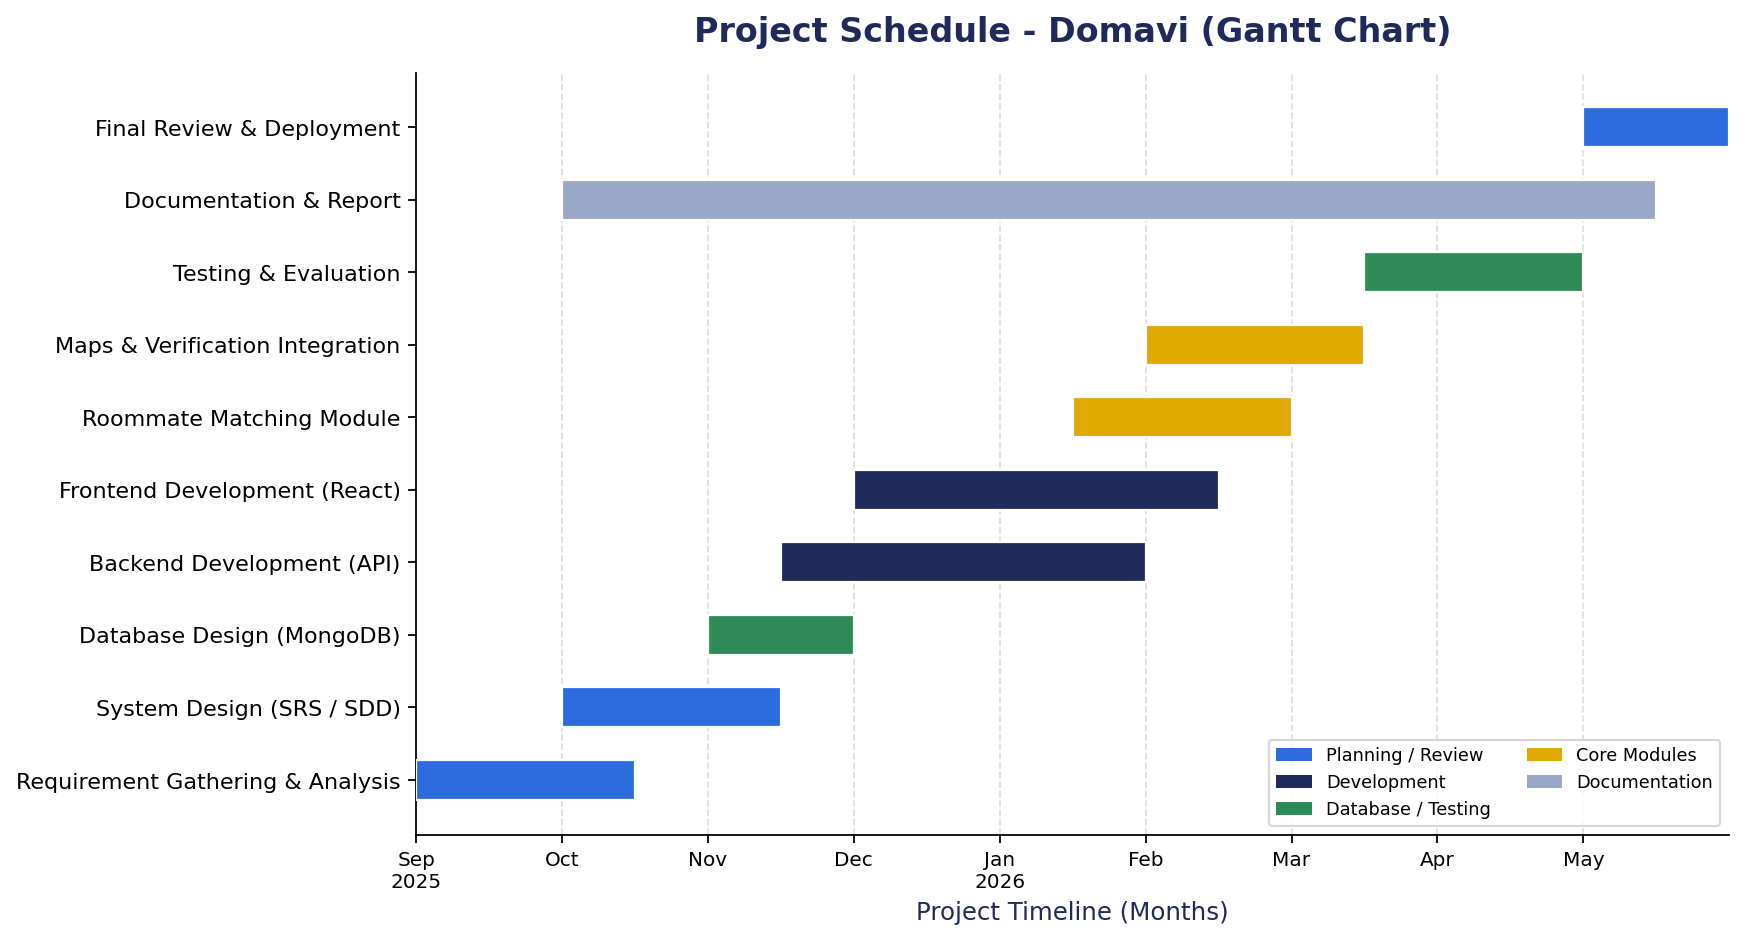
\includegraphics[width=\textwidth]{Figures/Gantt Chart.png}
\caption{Project Schedule (Gantt Chart) of the Domavi Platform}
\label{fig:gantt}
\end{figure}

%%%%%%%%%%%%%%%%%%%%%%%%%%%%%%%%%%%%%%%%%%%%%%%%%%%%%%
\section{Chapter Summary}
%%%%%%%%%%%%%%%%%%%%%%%%%%%%%%%%%%%%%%%%%%%%%%%%%%%%%%

This chapter introduced the background and context of the Domavi platform,
highlighting the high cost, fraud risk, and roommate incompatibility that
characterise the current micro-rental market for students and young
professionals in Pakistan. The vision and strategic objectives of the system
were outlined to establish its intended impact and innovation. A comparative
analysis of related systems identified key limitations in current solutions
such as general classifieds, property portals, international roommate
platforms, and informal social media groups. Project deliverables, system
constraints, selected technologies, and academic relevance were also discussed.

This chapter establishes the foundation for the detailed problem definition
presented in the next chapter.
  
% ==============================
% Chapter 2 – Problem Definition
% ==============================

\chapter{Problem Definition}
% --------------------------------
% 2.1 Problem Statement
% --------------------------------

\section{Problem Statement}

Students and young professionals seeking affordable shared accommodation in Pakistani cities face a rental market that is informal, opaque, and unsafe. Finding a single room or bed space near a university or workplace typically requires engaging local brokers who charge high commissions, or browsing unverified listings on general classified sites and social media groups where fraudulent advertisements and fake landlords are common. There is no reliable mechanism to confirm that a property exists, that the advertiser owns it, or that the parties involved are genuine. Compounding this, the selection of a roommate, an inherently social decision, is left entirely to chance, frequently resulting in conflict and stress. The affected stakeholders are tenants, who bear financial and security risks; genuine landlords, who lack a trustworthy channel to reach reliable tenants; and the wider community, which is denied a transparent housing marketplace. The problem is significant because it imposes avoidable financial cost, wasted time, exposure to fraud, and reduced quality of life on a large and growing population.

% --------------------------------
% 2.2 Proposed Solution Overview
% --------------------------------

\section{Proposed Solution Overview}

Domavi is a web-based micro-rental and roommate matching platform that directly addresses the weaknesses of the current system. It provides a dedicated marketplace for single rooms, bed spaces, and hostels, replacing scattered and irrelevant listings with a focused, well-structured catalogue. To establish trust, the platform enforces a multi-layer verification system covering email and phone confirmation, administrator-reviewed CNIC verification, and property ownership validation, thereby reducing fraud. An intelligent roommate matching engine scores potential roommates on lifestyle, preferences, budget, location, and schedule, transforming roommate selection from guesswork into a data-driven decision. Commute-based search powered by the Google Maps API allows users to find accommodation within walking distance of their destination. Finally, secure in-app messaging, structured booking requests, payment recording, and auto-generated digital rental agreements automate the rental lifecycle. The result is a safer, cheaper, faster, and more transparent rental experience.

% --------------------------------
% 2.3 Objectives of the Proposed System
% --------------------------------

\section{Objectives of the Proposed System}

The objectives of Domavi are defined to be specific, measurable, and directly aligned with the problems identified above. Each objective begins with an action verb and is achievable within the project constraints.

\vspace{0.3cm}

\textbf{Business Objectives (BO):}

\begin{itemize}
    \item BO-1: Develop a dedicated micro-rental marketplace that enables users to list, search, and book single rooms, bed spaces, and hostels.
    \item BO-2: Provide an intelligent roommate matching engine that ranks potential roommates by multi-factor compatibility to reduce living conflicts.
    \item BO-3: Ensure trust and safety through a multi-layer verification system covering identity, contact, and property ownership.
    \item BO-4: Improve accommodation discovery by offering commute-based geospatial search relative to universities and workplaces.
    \item BO-5: Automate the rental workflow through secure messaging, structured bookings, payment recording, and auto-generated digital rental agreements.
    \item BO-6: Provide administrators with effective tools to verify users, oversee payments, and monitor platform activity.
\end{itemize}

% --------------------------------
% 2.4 Scope of the System
% --------------------------------

\section{Scope of the System}

Domavi is a responsive web application targeting students and young professionals seeking shared accommodation, the landlords who offer such accommodation, and the administrators who govern the platform. The system includes user registration and role-based access for tenants, landlords, and administrators; creation and management of room, bed-space, and hostel listings with images, pricing, amenities, and location; verification of users and properties; commute-based and filter-based search; roommate profile creation and compatibility-based matching; in-app messaging; booking requests and status management; payment recording and confirmation; auto-generated digital rental agreements; and an administrative dashboard with analytics.

The system explicitly excludes full-house sales and commercial property transactions, live integration with a third-party payment gateway in the initial release, native mobile applications, and nationwide coverage beyond the initially targeted cities. These exclusions delineate the platform's coverage and are distinct from the operational limitations described in Chapter~1.

% --------------------------------
% 2.5 System Architecture and Modules
% --------------------------------

\section{System Architecture and Modules}

Domavi follows a layered, client-server architecture organised into a presentation layer, an application (business logic) layer, and a data layer. The presentation layer is a React single-page application that communicates with the backend exclusively through a RESTful API. The application layer, built on Node.js and Express.js, hosts modular controllers and services that implement business rules and enforce role-based access control. The data layer is a MongoDB database accessed through Mongoose models. External services, including the Google Maps API, cloud media storage, and an email service, are integrated through the application layer. This modular design promotes loose coupling, reusability, and independent development and testing of each module, and a high-level architecture diagram is presented in Chapter~4.

% --------------------------------
% 2.5.1 Module Descriptions
% --------------------------------

\subsection{Module 1: User and Profile Management}

This module handles registration, authentication, authorisation, and profile management for the three supported user roles: Tenant, Landlord, and Administrator. It issues and validates JWT-based sessions, enforces role-based access control, manages account status (pending, active, suspended), and supports email/phone confirmation and CNIC submission as part of the verification process.

\textbf{Functional Requirements:}

\begin{itemize}
    \item FE-1: The system shall allow users to register using valid credentials and a selected role.
    \item FE-2: The system shall authenticate users and issue a secure session token before granting access.
    \item FE-3: The system shall allow users to view and update their profile information.
    \item FE-4: The system shall enforce role-based access to protected resources.
\end{itemize}

\subsection{Module 2: Communication Module}

This module enables secure, in-app interaction between tenants and landlords. It supports conversation threads, real-time message exchange, and notification of relevant events such as booking updates, allowing parties to negotiate and coordinate without sharing personal contact details prematurely.

\textbf{Functional Requirements:}

\begin{itemize}
    \item FE-1: The system shall enable secure messaging between tenants and landlords.
    \item FE-2: The system shall generate notifications for booking and verification events.
    \item FE-3: The system shall maintain a persistent history of conversations and messages.
\end{itemize}

\subsection{Module 3: Property Listing and Search Module (Core)}

This module delivers the core value of the platform. It allows landlords to create and manage micro-rental listings and allows tenants to search and filter those listings, including commute-based proximity search using the Google Maps API. It directly addresses the discovery problem identified in Section~2.1.

\textbf{Functional Requirements:}

\begin{itemize}
    \item FE-1: The system shall allow landlords to create, update, and remove property listings.
    \item FE-2: The system shall allow tenants to search and filter listings by location, price, room type, and gender preference.
    \item FE-3: The system shall support commute-based search returning listings near a chosen location.
    \item FE-4: The system shall display only verified and active listings in public search results.
\end{itemize}

\subsection{Module 4: Booking, Payment, and Agreement Module}

This module manages the rental transaction lifecycle. Tenants submit booking requests, landlords accept or reject them, payments are recorded and confirmed, and a digital rental agreement is auto-generated as a PDF for the confirmed booking.

\textbf{Functional Requirements:}

\begin{itemize}
    \item FE-1: The system shall allow tenants to submit booking requests for available listings.
    \item FE-2: The system shall allow landlords to accept or reject booking requests.
    \item FE-3: The system shall record payment details and update payment status upon confirmation.
    \item FE-4: The system shall auto-generate a digital rental agreement for confirmed bookings.
\end{itemize}

\subsection{Module 5: Roommate Matching Module (Advanced)}

This module provides the platform's distinctive intelligent capability. Users complete a lifestyle and preference profile, and the matching engine computes a weighted compatibility score against other profiles, returning a ranked list of the most compatible potential roommates.

\textbf{Functional Requirements:}

\begin{itemize}
    \item FE-1: The system shall allow users to create and update a roommate lifestyle profile.
    \item FE-2: The system shall compute a weighted compatibility score between roommate profiles.
    \item FE-3: The system shall return a ranked list of top roommate matches for a given profile.
\end{itemize}

\subsection{Module 6: Administration Module}

This module gives administrators control over the platform. It supports reviewing and approving CNIC and ownership verification requests, managing user accounts and status, overseeing payments, and viewing platform analytics.

\textbf{Functional Requirements:}

\begin{itemize}
    \item FE-1: The system shall allow administrators to review and approve or reject verification requests.
    \item FE-2: The system shall allow administrators to manage user accounts and account status.
    \item FE-3: The system shall provide administrators with analytics on users, listings, bookings, and payments.
\end{itemize}

% --------------------------------
% 2.7 Assumptions and Dependencies
% --------------------------------

\section{Assumptions and Dependencies}

The design of Domavi rests on a number of assumptions and external dependencies that define its operating conditions.

\begin{itemize}
    \item The system assumes that users have access to a stable internet connection and a modern web browser.
    \item The system assumes that users possess basic digital literacy and provide truthful information during verification.
    \item The system depends on the continued availability and quota limits of the Google Maps API for geospatial features.
    \item The system depends on third-party cloud media storage for images and verification documents, and on an SMTP email service for notifications.
    \item The system requires administrator availability to process manual CNIC and ownership verification requests in a timely manner.
\end{itemize}

%%%%%%%%%%%%%%%%%%%%%%%%%%%%%%%%%%%%%%%%%%%%%%%%%%%%%%
\section{Chapter Summary}
%%%%%%%%%%%%%%%%%%%%%%%%%%%%%%%%%%%%%%%%%%%%%%%%%%%%%%

This chapter defined the core problem addressed by Domavi and outlined the
conceptual solution approach. Clear, measurable objectives were established to
ensure alignment with the identified challenges of cost, fraud, discovery, and
roommate incompatibility. The system scope and architectural overview were
presented to define structural boundaries and major modules, namely user and
profile management, communication, property listing and search, booking and
agreements, roommate matching, and administration. Key assumptions and
dependencies were also documented to clarify operational constraints.

This chapter provides the problem foundation and sets the direction for the
detailed requirement analysis and software design presented in the following chapters.
 
%%%%%%%%%%%%%%%%%%%%%%%%%%%%%%%%%%%%%%%%%%%%%%%%%%%%%%%%%%%%
% CHAPTER 3 – REQUIREMENT ANALYSIS
%%%%%%%%%%%%%%%%%%%%%%%%%%%%%%%%%%%%%%%%%%%%%%%%%%%%%%%%%%%%

\chapter{Requirement Analysis}

%===========================================================
\section{Introduction to Requirement Analysis}
%===========================================================

This chapter presents a structured and formal specification of the system requirements for the Domavi platform. The purpose of this chapter is to clearly define what the system shall accomplish before proceeding to the system design phase. The requirements documented here serve as a contractual foundation for implementation, validation, and system testing.

The requirement analysis includes requirement elicitation techniques, identification of user classes, use case modelling, functional requirements, non-functional requirements, and external interface requirements. All requirements are written in measurable and testable form using standard requirement engineering principles.

%===========================================================
\section{Requirement Elicitation Techniques}
%===========================================================

This section describes the techniques used to gather and refine the requirements of the Domavi platform. Requirement elicitation ensured that the platform's capabilities are aligned with the real needs of students, young professionals, and landlords.

Requirements for this project were identified using the following techniques:

\begin{itemize}
    \item Informal interviews and discussions with students and young professionals about their experiences finding rooms and roommates.
    \item Analysis of existing solutions such as OLX, Zameen.com, international roommate platforms, and social media housing groups to identify functional gaps.
    \item Literature review of micro-rental and roommate matching systems and their design approaches.
    \item Observation of the current, broker-driven rental workflow to understand pain points around cost, verification, and trust.
    \item Brainstorming and supervisor feedback sessions to refine and prioritise the proposed feature set.
\end{itemize}

%===========================================================
\section{User Classes and Characteristics}
%===========================================================

This section identifies the different categories of users who interact with the Domavi platform. Each user class is defined along with its responsibilities, access privileges, and technical proficiency. This classification supports the role-based access control enforced by the system.

\begin{table}[h]
\centering
\caption{User Classes and Characteristics}

\begin{tabularx}{\textwidth}{|p{3cm}|X|p{2.5cm}|}
\hline
\textbf{User Class} & \textbf{Description} & \textbf{Technical Level} \\
\hline
Tenant & Searches for rooms and roommates, submits booking requests, makes payments, messages landlords, and completes a roommate profile. The primary end user of the platform. & Basic \\
\hline
Landlord & Lists and manages rooms, bed spaces, and hostels, submits ownership and identity documents for verification, and accepts or rejects booking requests. & Basic to Intermediate \\
\hline
Administrator & Reviews and approves verification requests, manages user accounts and status, oversees payments, and monitors platform analytics. & Advanced \\
\hline
External Service & Third-party systems integrated with the platform, including the Google Maps API, cloud media storage, and the email service. & Technical \\
\hline
\end{tabularx}

\end{table}

%===========================================================
\section{System Overview}
%===========================================================

Domavi operates within a layered, client-server architecture designed to support secure, role-based interaction between user interfaces, business logic, and data storage. The React-based presentation layer communicates with a Node.js and Express.js application layer through a RESTful API, and the application layer persists data in a MongoDB database via Mongoose models. The system boundary encompasses all internal modules, namely user and profile management, property listing and search, roommate matching, booking, payment, agreement generation, messaging, and administration, together with the integrated external services for mapping, media storage, and email. Role-based access control governs every protected interaction, ensuring that tenants, landlords, and administrators can only perform actions appropriate to their role.

%===========================================================
\section{Use Case Model}
%===========================================================

The use case model represents the high-level interactions between the actors and the functionalities of the Domavi platform. It defines the system boundary and captures functional behaviour from the perspective of each user.

%===========================================================
\subsection{Use Case Diagram}
%===========================================================

\begin{figure}[h]
\centering
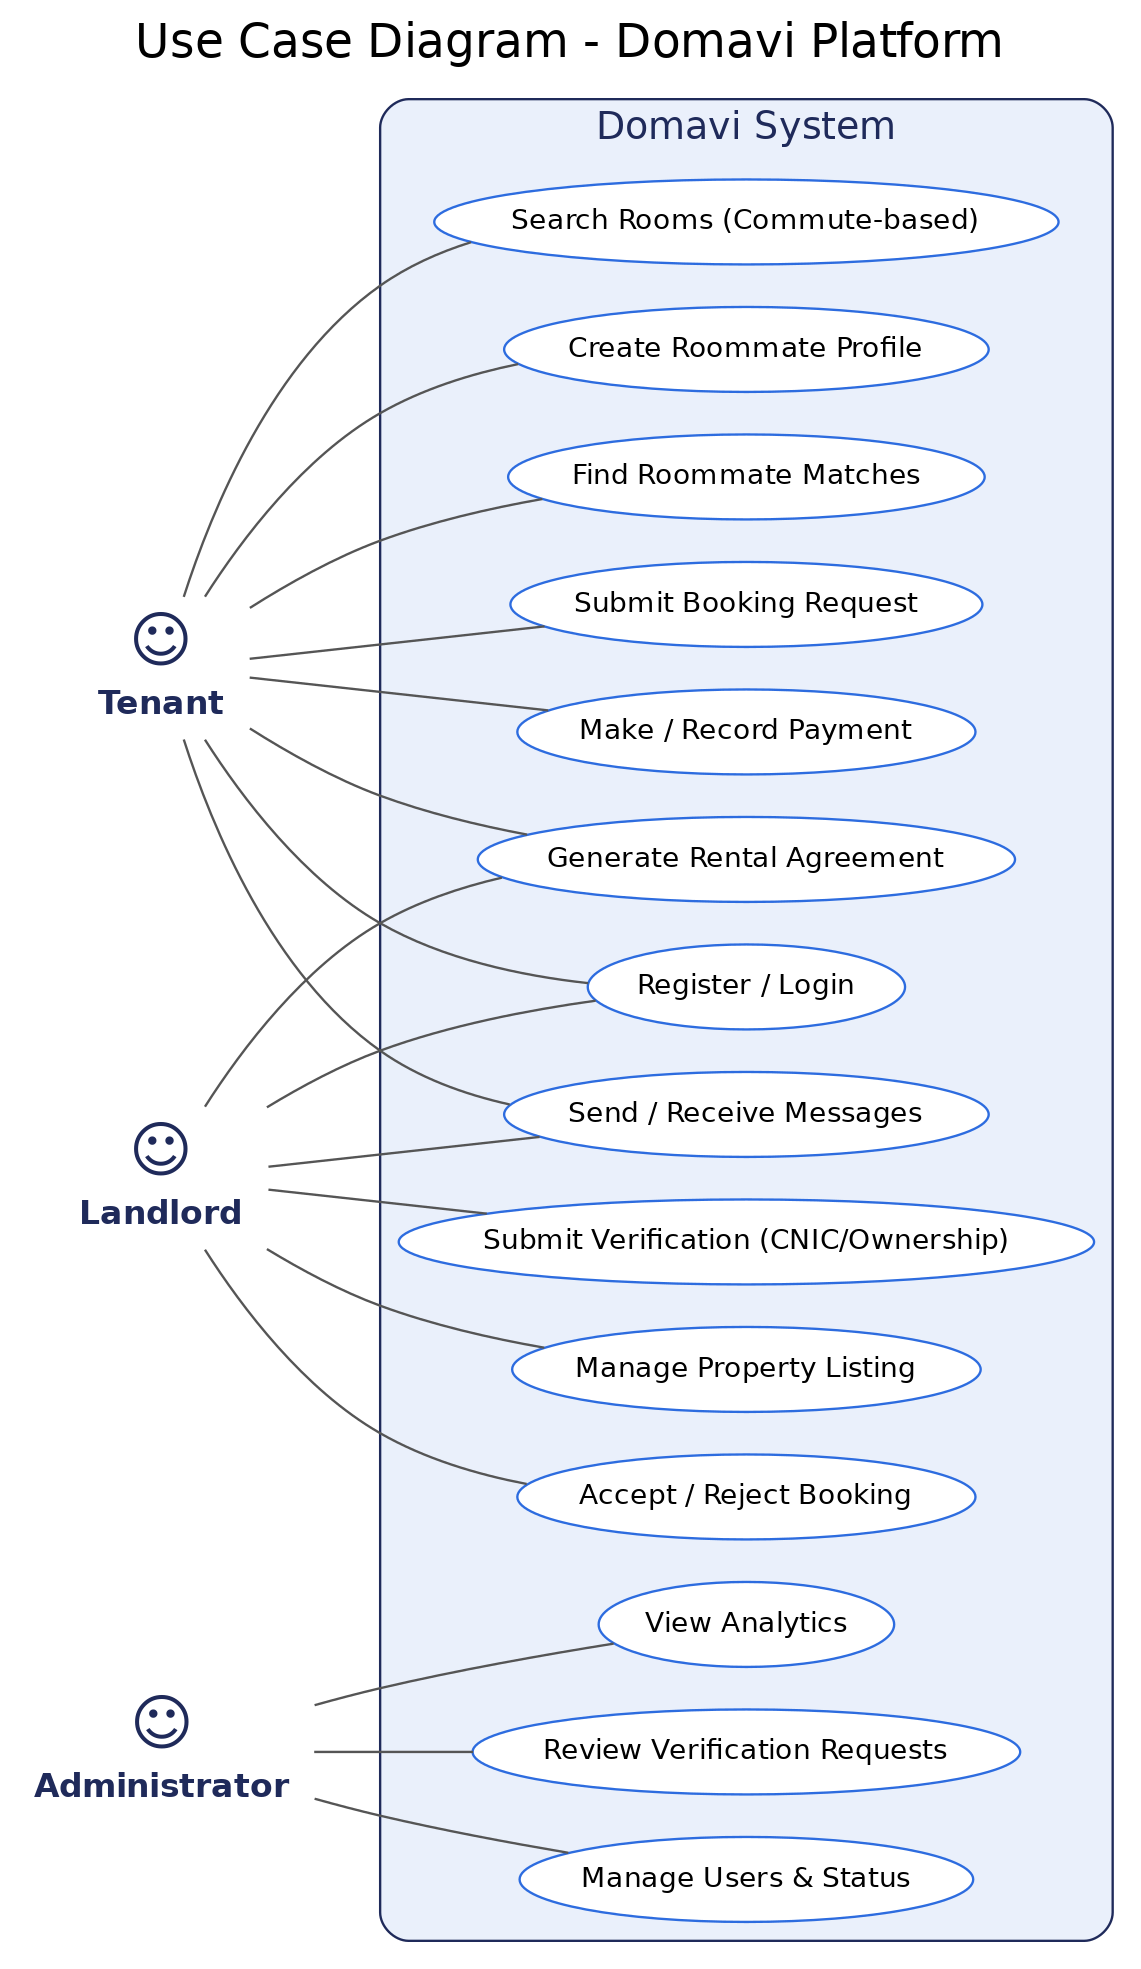
\includegraphics[width=0.6\textwidth]{Figures/usecase_diagram.png}
\caption{Use Case Diagram of the Domavi Platform}
\label{fig:usecase}
\end{figure}

The diagram above illustrates the interaction between the three primary actors, Tenant, Landlord, and Administrator, and the major system functionalities. Common functionality such as registration, login, and verification is shared through \textit{include} relationships, while optional behaviour such as roommate matching extends the core search experience. \textit{(This is a sample diagram from the template; replace it with the finalised Domavi use case diagram before submission.)}

%===========================================================
\subsection{Use Case Descriptions}
%===========================================================

This section provides detailed tabular specifications of the major use cases. These use cases form the basis for deriving the functional requirements presented later in this chapter.

\subsubsection{Module 1: User and Verification}

Below are detailed use cases for registration and verification.

\begin{table}[h]
\centering
\caption{UC-1.1: User Registration}

\begin{tabularx}{\textwidth}{
|>{\raggedright\arraybackslash}p{3.5cm}
|>{\raggedright\arraybackslash}X|}

\hline
\textbf{Use Case ID} & UC-1.1 \\ \hline
\textbf{Use Case Name} & User Registration \\ \hline
\textbf{Actors} & Tenant, Landlord \\ \hline
\textbf{Description} & A new user creates an account and selects a role (tenant or landlord). \\ \hline
\textbf{Trigger} & User selects the ``Sign Up'' option. \\ \hline
\textbf{Preconditions} & User is not already registered with the provided email. \\ \hline
\textbf{Postconditions} & A new account is created with status \textit{pending} and a verification email is sent. \\ \hline
\textbf{Normal Flow} &
\begin{enumerate}
    \item User enters name, email, password, and role.
    \item System validates the input fields.
    \item System creates the account and stores the hashed password.
    \item System sends an email verification link.
    \item Confirmation message is displayed.
\end{enumerate}
\\ \hline
\textbf{Alternative Flow} &
If the email already exists or validation fails, the system displays an appropriate error message.
\\ \hline

\end{tabularx}

\end{table}

\begin{table}[h]
\centering
\caption{UC-1.2: CNIC and Ownership Verification}

\begin{tabularx}{\textwidth}{
|>{\raggedright\arraybackslash}p{3.5cm}
|>{\raggedright\arraybackslash}X|}

\hline
\textbf{Use Case ID} & UC-1.2 \\ \hline
\textbf{Use Case Name} & CNIC and Ownership Verification \\ \hline
\textbf{Actors} & Landlord, Administrator \\ \hline
\textbf{Description} & A landlord submits identity and ownership documents, which an administrator reviews and approves or rejects. \\ \hline
\textbf{Trigger} & Landlord uploads CNIC and ownership proof. \\ \hline
\textbf{Preconditions} & Landlord is registered and logged in. \\ \hline
\textbf{Postconditions} & The verification request is approved or rejected and the user/property status is updated accordingly. \\ \hline
\textbf{Normal Flow} &
\begin{enumerate}
    \item Landlord uploads required documents.
    \item System stores the documents securely and creates a verification request.
    \item Administrator reviews the documents.
    \item Administrator approves or rejects the request.
    \item System updates the verification status and notifies the landlord.
\end{enumerate}
\\ \hline
\textbf{Alternative Flow} &
If the documents are invalid or unclear, the administrator rejects the request with a reason.
\\ \hline

\end{tabularx}

\end{table}

\subsubsection{Module 2: Property and Search}

\begin{table}[h]
\centering
\caption{UC-2.1: Create Property Listing}

\begin{tabularx}{\textwidth}{
|>{\raggedright\arraybackslash}p{3.5cm}
|>{\raggedright\arraybackslash}X|}

\hline
\textbf{Use Case ID} & UC-2.1 \\ \hline
\textbf{Use Case Name} & Create Property Listing \\ \hline
\textbf{Actors} & Landlord \\ \hline
\textbf{Description} & A verified landlord creates a listing for a room, bed space, or hostel. \\ \hline
\textbf{Trigger} & Landlord selects ``Add Property''. \\ \hline
\textbf{Preconditions} & Landlord is logged in and verified. \\ \hline
\textbf{Postconditions} & A new listing is created with status \textit{pending\_verification}. \\ \hline
\textbf{Normal Flow} &
\begin{enumerate}
    \item Landlord enters title, description, type, price, amenities, and location.
    \item Landlord uploads property images.
    \item System validates and geocodes the location.
    \item System saves the listing for review.
\end{enumerate}
\\ \hline
\textbf{Alternative Flow} &
If required fields are missing, the system prompts the landlord to complete them.
\\ \hline

\end{tabularx}

\end{table}

\begin{table}[h]
\centering
\caption{UC-2.2: Commute-Based Property Search}

\begin{tabularx}{\textwidth}{
|>{\raggedright\arraybackslash}p{3.5cm}
|>{\raggedright\arraybackslash}X|}

\hline
\textbf{Use Case ID} & UC-2.2 \\ \hline
\textbf{Use Case Name} & Commute-Based Property Search \\ \hline
\textbf{Actors} & Tenant \\ \hline
\textbf{Description} & A tenant searches for listings near a chosen university or workplace using filters. \\ \hline
\textbf{Trigger} & Tenant enters a location and search criteria. \\ \hline
\textbf{Preconditions} & Active and verified listings exist in the database. \\ \hline
\textbf{Postconditions} & A ranked list of nearby matching listings is displayed. \\ \hline
\textbf{Normal Flow} &
\begin{enumerate}
    \item Tenant enters a target location and filters (price, type, gender preference).
    \item System geocodes the location via the Maps API.
    \item System performs a geospatial query against active listings.
    \item System returns and displays matching listings on a map and list.
\end{enumerate}
\\ \hline
\textbf{Alternative Flow} &
If no listings match, the system displays an empty-state message with suggestions.
\\ \hline

\end{tabularx}

\end{table}

\subsubsection{Module 3: Booking and Roommate Matching}

\begin{table}[h]
\centering
\caption{UC-3.1: Submit Booking Request}

\begin{tabularx}{\textwidth}{
|>{\raggedright\arraybackslash}p{3.5cm}
|>{\raggedright\arraybackslash}X|}

\hline
\textbf{Use Case ID} & UC-3.1 \\ \hline
\textbf{Use Case Name} & Submit Booking Request \\ \hline
\textbf{Actors} & Tenant, Landlord \\ \hline
\textbf{Description} & A tenant requests to book a listing; the landlord accepts or rejects the request. \\ \hline
\textbf{Trigger} & Tenant selects ``Request Booking''. \\ \hline
\textbf{Preconditions} & Tenant is logged in and the listing is active. \\ \hline
\textbf{Postconditions} & A booking record is created with status \textit{pending} and the landlord is notified. \\ \hline
\textbf{Normal Flow} &
\begin{enumerate}
    \item Tenant selects move-in date and submits the request.
    \item System creates a booking with pending status.
    \item Landlord reviews and accepts or rejects the request.
    \item System updates the booking status and notifies the tenant.
\end{enumerate}
\\ \hline
\textbf{Alternative Flow} &
If the landlord rejects the request, the tenant is notified and may search for alternatives.
\\ \hline

\end{tabularx}

\end{table}

\begin{table}[h]
\centering
\caption{UC-3.2: Find Roommate Matches}

\begin{tabularx}{\textwidth}{
|>{\raggedright\arraybackslash}p{3.5cm}
|>{\raggedright\arraybackslash}X|}

\hline
\textbf{Use Case ID} & UC-3.2 \\ \hline
\textbf{Use Case Name} & Find Roommate Matches \\ \hline
\textbf{Actors} & Tenant \\ \hline
\textbf{Description} & A tenant requests a ranked list of compatible roommates based on their lifestyle profile. \\ \hline
\textbf{Trigger} & Tenant opens the ``Roommate Matches'' page. \\ \hline
\textbf{Preconditions} & Tenant has completed a roommate lifestyle profile. \\ \hline
\textbf{Postconditions} & A ranked list of compatible roommate profiles is displayed. \\ \hline
\textbf{Normal Flow} &
\begin{enumerate}
    \item System retrieves the tenant's roommate profile.
    \item System computes weighted compatibility scores against other profiles.
    \item System sorts candidates by score.
    \item System displays the top matches with their compatibility scores.
\end{enumerate}
\\ \hline
\textbf{Alternative Flow} &
If the profile is incomplete, the system prompts the tenant to complete it first.
\\ \hline

\end{tabularx}

\end{table}

%===========================================================
\subsection{Event-Response Table}
%===========================================================

The event-response table defines how the system reacts to significant internal and external events.

\begin{table}[h]
\centering
\caption{Event-Response Table}

\begin{tabularx}{\textwidth}{
|>{\raggedright\arraybackslash}p{3.5cm}
|>{\raggedright\arraybackslash}p{3cm}
|>{\raggedright\arraybackslash}X|}

\hline
\textbf{Event} & \textbf{Source} & \textbf{System Response} \\ \hline

User Login Attempt & Tenant / Landlord / Admin & Validate credentials and grant or deny access based on role. \\ \hline

Document Upload & Landlord & Store CNIC/ownership document securely and create a verification request. \\ \hline

Property Search & Tenant & Geocode the location and return nearby active listings. \\ \hline

Booking Request & Tenant & Create a pending booking and notify the landlord. \\ \hline

Roommate Match Request & Tenant & Compute weighted compatibility scores and return ranked matches. \\ \hline

Payment Submission & Tenant & Record payment details and set status pending until admin confirmation. \\ \hline

\end{tabularx}

\end{table}

%===========================================================
\section{Functional Requirements}
%===========================================================

Functional requirements define the core services and behaviours that the system shall provide. These requirements are derived directly from the use case model presented in Section~3.5. Each requirement is uniquely identified, measurable, and written using formal specification language, and the requirements are categorised by system module.

%===========================================================
\subsection{Module 1: User and Verification Management}
%===========================================================

\subsubsection{FR-1.1 User Registration}

\begin{table}[h]
\centering
\caption{Functional Requirement -- User Registration}

\begin{tabularx}{\textwidth}{|p{3cm}|X|}
\hline
\textbf{Identifier} & FR-1.1 \\
\hline
\textbf{Title} & User Registration \\
\hline
\textbf{Requirement} & The system shall allow users to create an account by providing a name, valid email, password, and role (tenant or landlord). \\
\hline
\textbf{Source} & Stakeholder Requirement \\
\hline
\textbf{Rationale} & Enables authorised, role-based access to platform services. \\
\hline
\textbf{Dependencies} & Database connectivity, email service \\
\hline
\textbf{Priority} & High \\
\hline
\end{tabularx}

\end{table}

\subsubsection{FR-1.2 Multi-Layer Verification}

\begin{table}[h]
\centering
\caption{Functional Requirement -- Multi-Layer Verification}

\begin{tabularx}{\textwidth}{|p{3cm}|X|}
\hline
\textbf{Identifier} & FR-1.2 \\
\hline
\textbf{Title} & Multi-Layer Verification \\
\hline
\textbf{Requirement} & The system shall support email/phone confirmation and allow landlords to submit CNIC and ownership documents for administrator review. \\
\hline
\textbf{Source} & Business Objective BO-3 \\
\hline
\textbf{Rationale} & Establishes trust and reduces fraud on the platform. \\
\hline
\textbf{Dependencies} & Media storage, administration module \\
\hline
\textbf{Priority} & High \\
\hline
\end{tabularx}

\end{table}

%===========================================================
\subsection{Module 2: Property Listing and Search}
%===========================================================

\subsubsection{FR-2.1 Manage Property Listings}

\begin{table}[h]
\centering
\caption{Functional Requirement -- Manage Property Listings}

\begin{tabularx}{\textwidth}{|p{3cm}|X|}
\hline
\textbf{Identifier} & FR-2.1 \\
\hline
\textbf{Title} & Manage Property Listings \\
\hline
\textbf{Requirement} & The system shall allow verified landlords to create, update, and remove listings for rooms, bed spaces, and hostels, including images, price, amenities, and location. \\
\hline
\textbf{Source} & Business Objective BO-1 \\
\hline
\textbf{Rationale} & Provides the supply side of the micro-rental marketplace. \\
\hline
\textbf{Dependencies} & Media storage, Maps API (geocoding) \\
\hline
\textbf{Priority} & High \\
\hline
\end{tabularx}

\end{table}

\subsubsection{FR-2.2 Commute-Based Search}

\begin{table}[h]
\centering
\caption{Functional Requirement -- Commute-Based Search}

\begin{tabularx}{\textwidth}{|p{3cm}|X|}
\hline
\textbf{Identifier} & FR-2.2 \\
\hline
\textbf{Title} & Commute-Based Search \\
\hline
\textbf{Requirement} & The system shall allow tenants to search and filter active, verified listings by proximity to a chosen location, price, room type, and gender preference. \\
\hline
\textbf{Source} & Business Objective BO-4 \\
\hline
\textbf{Rationale} & Enables efficient discovery of relevant accommodation near study or work. \\
\hline
\textbf{Dependencies} & Geospatial index, Maps API \\
\hline
\textbf{Priority} & High \\
\hline
\end{tabularx}

\end{table}

%===========================================================
\subsection{Module 3: Booking, Payment, and Agreements}
%===========================================================

\subsubsection{FR-3.1 Booking Management}

\begin{table}[h]
\centering
\caption{Functional Requirement -- Booking Management}

\begin{tabularx}{\textwidth}{|p{3cm}|X|}
\hline
\textbf{Identifier} & FR-3.1 \\
\hline
\textbf{Title} & Booking Management \\
\hline
\textbf{Requirement} & The system shall allow tenants to submit booking requests and allow landlords to accept or reject them, updating the booking status accordingly. \\
\hline
\textbf{Source} & Business Objective BO-5 \\
\hline
\textbf{Rationale} & Structures and tracks the rental transaction. \\
\hline
\textbf{Dependencies} & Property module, notification service \\
\hline
\textbf{Priority} & High \\
\hline
\end{tabularx}

\end{table}

\subsubsection{FR-3.2 Digital Rental Agreement}

\begin{table}[h]
\centering
\caption{Functional Requirement -- Digital Rental Agreement}

\begin{tabularx}{\textwidth}{|p{3cm}|X|}
\hline
\textbf{Identifier} & FR-3.2 \\
\hline
\textbf{Title} & Digital Rental Agreement \\
\hline
\textbf{Requirement} & The system shall auto-generate a digital rental agreement in PDF format for each confirmed booking, recording the tenant, landlord, property, and terms. \\
\hline
\textbf{Source} & Business Objective BO-5 \\
\hline
\textbf{Rationale} & Automates documentation and provides a verifiable record. \\
\hline
\textbf{Dependencies} & Booking module, PDF generation library \\
\hline
\textbf{Priority} & Medium \\
\hline
\end{tabularx}

\end{table}

%===========================================================
\subsection{Module 4: Roommate Matching}
%===========================================================

\subsubsection{FR-4.1 Roommate Compatibility Matching}

\begin{table}[h]
\centering
\caption{Functional Requirement -- Roommate Compatibility Matching}

\begin{tabularx}{\textwidth}{|p{3cm}|X|}
\hline
\textbf{Identifier} & FR-4.1 \\
\hline
\textbf{Title} & Roommate Compatibility Matching \\
\hline
\textbf{Requirement} & The system shall compute a weighted compatibility score between roommate profiles across lifestyle, preferences, budget, location, and schedule, and return a ranked list of top matches. \\
\hline
\textbf{Source} & Business Objective BO-2 \\
\hline
\textbf{Rationale} & Replaces the roommate ``gamble'' with data-driven matching. \\
\hline
\textbf{Dependencies} & Roommate profile data \\
\hline
\textbf{Priority} & High \\
\hline
\end{tabularx}

\end{table}

%===========================================================
\subsection{Module 5: Communication and Administration}
%===========================================================

\subsubsection{FR-5.1 Secure Messaging}

\begin{table}[h]
\centering
\caption{Functional Requirement -- Secure Messaging}

\begin{tabularx}{\textwidth}{|p{3cm}|X|}
\hline
\textbf{Identifier} & FR-5.1 \\
\hline
\textbf{Title} & Secure Messaging \\
\hline
\textbf{Requirement} & The system shall enable secure, in-app messaging between tenants and landlords and maintain a persistent conversation history. \\
\hline
\textbf{Source} & Stakeholder Requirement \\
\hline
\textbf{Rationale} & Allows coordination without prematurely exposing personal contact details. \\
\hline
\textbf{Dependencies} & Authentication module \\
\hline
\textbf{Priority} & Medium \\
\hline
\end{tabularx}

\end{table}

\subsubsection{FR-5.2 Administration and Analytics}

\begin{table}[h]
\centering
\caption{Functional Requirement -- Administration and Analytics}

\begin{tabularx}{\textwidth}{|p{3cm}|X|}
\hline
\textbf{Identifier} & FR-5.2 \\
\hline
\textbf{Title} & Administration and Analytics \\
\hline
\textbf{Requirement} & The system shall allow administrators to review verification requests, manage user accounts and status, oversee payments, and view platform analytics. \\
\hline
\textbf{Source} & Business Objective BO-6 \\
\hline
\textbf{Rationale} & Provides governance, oversight, and operational insight. \\
\hline
\textbf{Dependencies} & All modules \\
\hline
\textbf{Priority} & High \\
\hline
\end{tabularx}

\end{table}

%===========================================================
\section{Non-Functional Requirements}
%===========================================================

Non-functional requirements define the quality attributes that describe how the system performs. These requirements are measurable and support reliability, usability, performance, security, and maintainability.

%===========================================================
\subsection{Performance Requirements}
%===========================================================

\begin{itemize}
\item PER-1: The system shall load the main dashboard and search results within 3 seconds under normal operating conditions.
\item PER-2: The system shall return roommate match results within an acceptable latency for a typical candidate pool.
\item PER-3: The system shall support multiple concurrent users as defined in the project scope without significant degradation.
\item PER-4: Geospatial search queries shall be optimised through appropriate indexing to ensure responsive results.
\end{itemize}

%===========================================================
\subsection{Security Requirements}
%===========================================================

\begin{itemize}
\item SEC-1: The system shall implement secure authentication using JSON Web Tokens.
\item SEC-2: Passwords shall be stored using a secure hashing algorithm with salting.
\item SEC-3: Sensitive data shall be transmitted over HTTPS.
\item SEC-4: Role-based access control shall be enforced for every protected resource.
\item SEC-5: Verification documents (CNIC, ownership proof) shall be stored securely and accessible only to authorised administrators.
\end{itemize}

%===========================================================
\subsection{Reliability Requirements}
%===========================================================

\begin{itemize}
\item REL-1: The system shall aim to maintain high availability with at least 99\% uptime.
\item REL-2: System failures shall not result in loss of booking, payment, or agreement data.
\item REL-3: Backup and recovery mechanisms shall be in place for the database.
\end{itemize}

%===========================================================
\subsection{Usability Requirements}
%===========================================================

\begin{itemize}
\item USE-1: The interface shall be intuitive and easy to navigate for users with basic digital literacy.
\item USE-2: Clear and meaningful error messages shall be displayed for invalid actions.
\item USE-3: The system shall follow consistent UI/UX design principles across all pages.
\item USE-4: The application shall be fully responsive across desktop and mobile browsers.
\end{itemize}

%===========================================================
\subsection{Scalability Requirements}
%===========================================================

\begin{itemize}
\item SCA-1: The system shall support a growing number of users and listings.
\item SCA-2: The architecture shall allow horizontal or vertical scaling of the application and database.
\item SCA-3: The database design shall support large volumes of listings and roommate profiles.
\end{itemize}

%===========================================================
\subsection{Maintainability Requirements}
%===========================================================

\begin{itemize}
\item MAIN-1: The system shall follow a modular architecture with clear separation of concerns.
\item MAIN-2: Source code shall be written in TypeScript and documented for clarity.
\item MAIN-3: Future features shall be integrable without major restructuring of existing modules.
\end{itemize}

%===========================================================
\section{External Interface Requirements}
%===========================================================

This section defines how the Domavi platform interacts with external entities including users, hardware devices, software systems, and communication networks.

%===========================================================
\subsection{User Interface Requirements}
%===========================================================

\begin{itemize}
\item UI-1: The system shall provide a graphical web interface accessible from modern browsers.
\item UI-2: Standard, readable font sizes shall be used throughout (12--14pt body text).
\item UI-3: The layout shall be responsive across desktop, tablet, and mobile devices.
\item UI-4: Navigation shall remain consistent and role-appropriate across all modules.
\end{itemize}

%===========================================================
\subsection{Hardware Interface Requirements}
%===========================================================

\begin{itemize}
\item HI-1: The system shall operate on standard computing devices with an internet connection.
\item HI-2: The application shall function on devices running modern web browsers without specialised hardware.
\item HI-3: Server hosting shall provide sufficient compute and storage for the database and media.
\end{itemize}

%===========================================================
\subsection{Software Interface Requirements}
%===========================================================

\begin{itemize}
\item SI-1: The system shall interact with a MongoDB database through the Mongoose object data modelling layer.
\item SI-2: The system shall integrate the Google Maps API for geocoding and map display.
\item SI-3: The system shall integrate cloud media storage for images and verification documents.
\item SI-4: The system shall integrate an SMTP email service for verification and notifications.
\end{itemize}

%===========================================================
\subsection{Communication Interface Requirements}
%===========================================================

\begin{itemize}
\item CI-1: The system shall use HTTPS for secure client-server communication.
\item CI-2: RESTful APIs shall be used for all backend communication.
\item CI-3: Real-time messaging shall be supported for in-app conversations.
\item CI-4: All API requests to protected endpoints shall carry a valid authentication token.
\end{itemize}

%===========================================================
\section{Assumptions and Dependencies}
%===========================================================

This section lists the assumptions made during requirement analysis and the external dependencies on which the system relies.

\begin{itemize}
\item The system assumes stable internet connectivity for all online operations.
\item Third-party services (Google Maps API, cloud media storage, email service) are assumed to remain available and within quota.
\item Users are assumed to provide truthful information and possess basic digital literacy.
\item Administrators are assumed to be available to process manual verification requests in a timely manner.
\end{itemize}

%===========================================================
\section{Requirement Traceability Matrix}
%===========================================================

This matrix maps project objectives to use cases and functional requirements to ensure alignment and completeness.

\begin{table}[h]
\centering
\caption{Requirement Traceability Matrix}

\begin{tabularx}{\textwidth}{|p{2cm}|p{3cm}|X|}
\hline
\textbf{Objective} & \textbf{Use Case} & \textbf{Functional Requirement} \\ \hline
BO-1 & UC-2.1 & FR-2.1 \\ \hline
BO-2 & UC-3.2 & FR-4.1 \\ \hline
BO-3 & UC-1.2 & FR-1.2 \\ \hline
BO-4 & UC-2.2 & FR-2.2 \\ \hline
BO-5 & UC-3.1 & FR-3.1, FR-3.2 \\ \hline
BO-6 & UC-1.2 & FR-5.2 \\ \hline
\end{tabularx}

\end{table}

%===========================================================
\section*{Chapter Summary}
%===========================================================

This chapter presented a structured requirement analysis of the Domavi platform.
It defined the requirement elicitation techniques, the user classes (tenant,
landlord, administrator, and external services), and a use case model with
detailed use case specifications for registration, verification, listing,
search, booking, and roommate matching. Functional requirements were specified
module by module, followed by measurable non-functional requirements covering
performance, security, reliability, usability, scalability, and maintainability.
External interface requirements and a traceability matrix linking objectives to
requirements were also included. These requirements form the formal foundation
for the system design presented in the next chapter.

\chapter{Software Design}

\section{Introduction to Software Design}

This chapter presents the detailed software design of the Property Rental System platform. It translates the requirements identified in Chapter~3 into structured architectural, behavioural, and data models. The purpose of this chapter is to provide a clear blueprint for system implementation, ensuring maintainability, scalability, and modular development.

The chapter covers the design methodology and software process model, a high-level system overview and architecture, UML behavioural and structural models, data flow diagrams, and the database design including the entity relationship model, schema, and data dictionary for the platform's MongoDB collections.

%%%%%%%%%%%%%%%%%%%%%%%%%%%%%%%%%%%%%%%%%%%%%%%%%%%%%%
\section{Design Methodology and Software Process Model}

\subsection{Design Methodology}

Property Rental System follows an object-oriented, layered design methodology combined with the Model-View-Controller pattern on the backend. The system is divided into a presentation layer (React client), an application layer (Express controllers and services), and a data layer (MongoDB through Mongoose models). Within the application layer, controllers handle request and response concerns while services encapsulate business logic, giving a clear separation of concerns.

This methodology was selected because it suits a web application with multiple user roles and evolving features. It enforces loose coupling between layers, promotes reuse of services across controllers, and allows each module to be developed and tested independently. The design adheres to established principles including Separation of Concerns, the DRY (Don't Repeat Yourself) principle, and SOLID object-oriented design guidelines, particularly single-responsibility services and dependency inversion through well-defined interfaces.

\subsection{Software Process Model}

The project follows the \textbf{Agile (iterative and incremental)} process model. Agile was selected because the requirements were refined progressively through stakeholder feedback and supervisor reviews, and because the platform's features, such as listing management, search, booking, and roommate matching, lend themselves naturally to incremental delivery. Development proceeded in short iterations, each delivering a working slice of functionality that was tested and reviewed before the next iteration began. Testing and validation were integrated continuously rather than deferred to a single final phase, allowing defects to be identified and corrected early.

%%%%%%%%%%%%%%%%%%%%%%%%%%%%%%%%%%%%%%%%%%%%%%%%%%%%%%
\section{System Overview}

This section provides a high-level overview of the system components and their interactions with external entities. At the boundary, three human actors, the tenant, the landlord, and the administrator, interact with the Property Rental System platform, while three external services, the Google Maps API, cloud media storage, and the email service, support the platform's operation. The context diagram below depicts the system as a single process exchanging data with these external entities.

\begin{figure}[h]
\centering
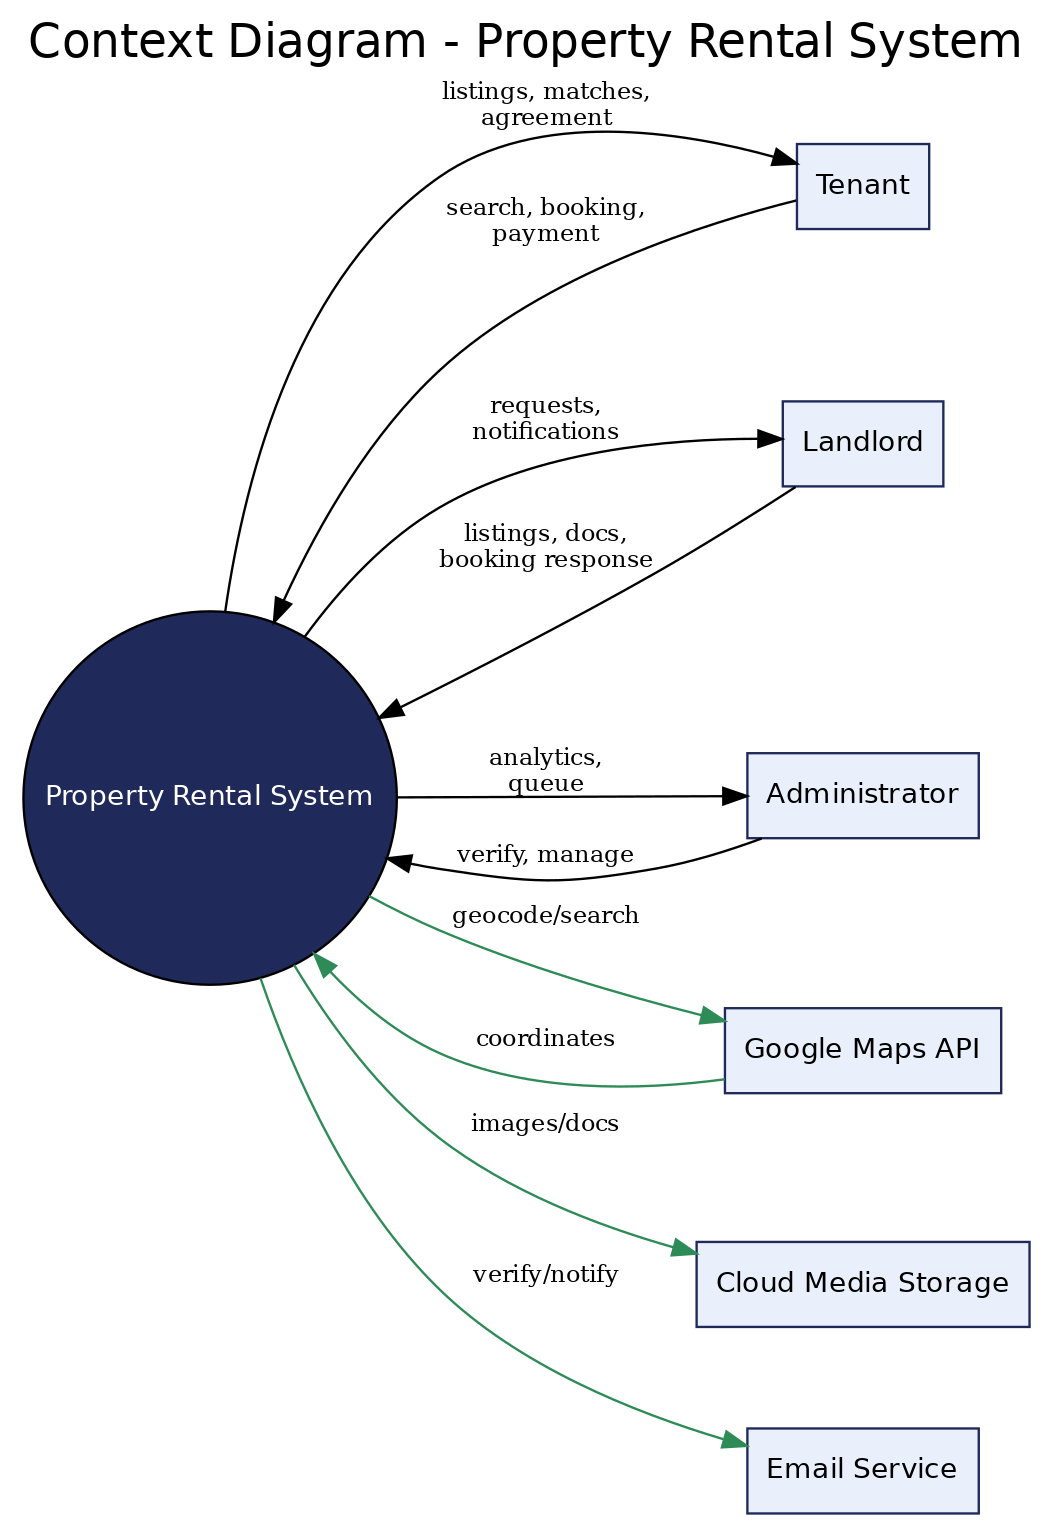
\includegraphics[width=0.9\textwidth]{Figures/Context Diagram.png}
\caption{Context Diagram of the Property Rental System Platform}
\label{fig:context}
\end{figure}

\noindent\textit{(The figure above is a sample from the template; replace it with the finalised Property Rental System context diagram before submission.)} The diagram shows the system boundary, the human actors who submit requests and receive responses, and the third-party services that the platform calls for mapping, storage, and email.

%%%%%%%%%%%%%%%%%%%%%%%%%%%%%%%%%%%%%%%%%%%%%%%%%%%%%%
\section{Architectural Design}

Property Rental System adopts a three-layer client-server architecture. The presentation layer is a React single-page application built with Vite and styled with Tailwind CSS, using Zustand for client-side state. It communicates with the backend solely through a RESTful API over HTTPS. The application layer is a Node.js and Express.js server organised into routes, controllers, and services; it enforces authentication and role-based access control through middleware and implements all business logic in dedicated service classes such as the authentication, property, booking, payment, chat, agreement, and roommate-matching services. The data layer is a MongoDB database accessed through Mongoose models, complemented by external integrations for geospatial search, media storage, and email.

\begin{figure}[h]
\centering
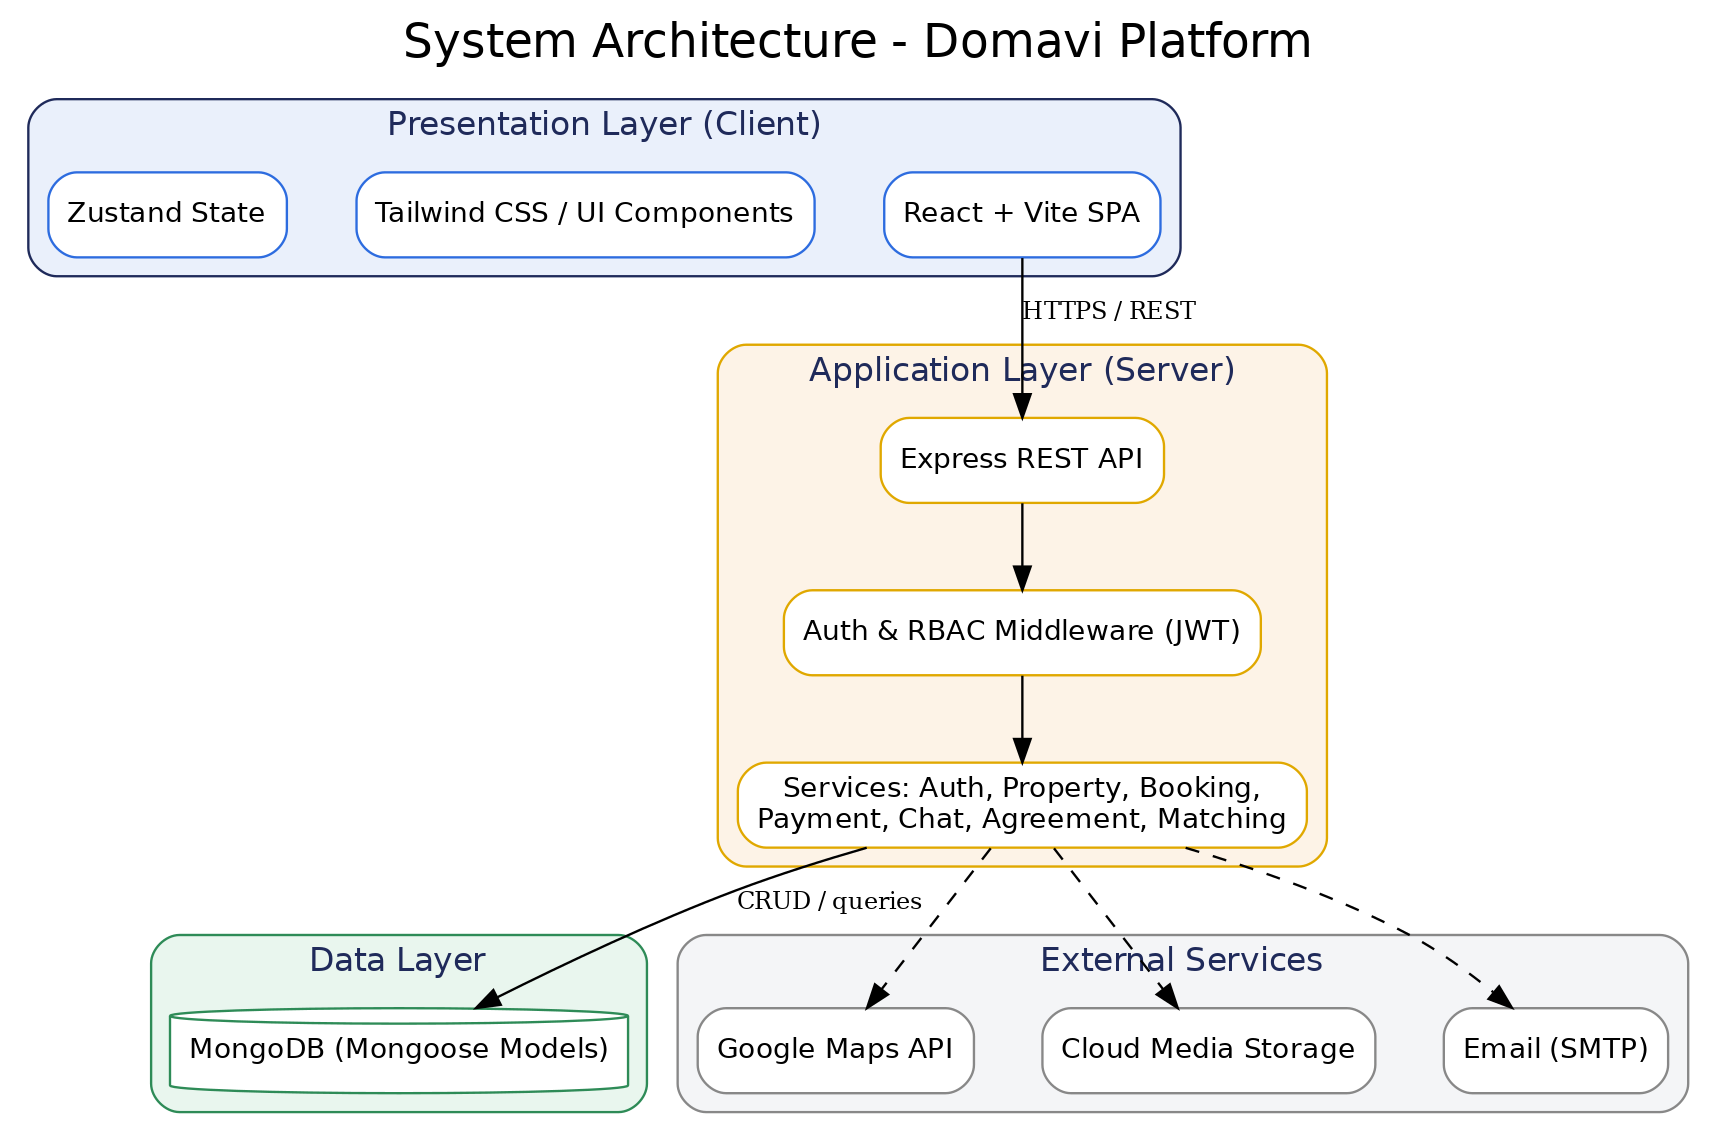
\includegraphics[width=0.9\textwidth]{Figures/Architecture Diagram.png}
\caption{System Architecture of the Property Rental System Platform}
\label{fig:arch}
\end{figure}

\noindent\textit{(Sample template figure; replace with the finalised Property Rental System architecture diagram.)} The presentation layer issues API requests; the API layer authenticates and authorises each request, delegates to the appropriate service, and the service interacts with the data layer and external services. Responses flow back through the same layers, keeping the frontend decoupled from data and integration concerns.

%%%%%%%%%%%%%%%%%%%%%%%%%%%%%%%%%%%%%%%%%%%%%%%%%%%%%%
\section{Design Models}

This section presents detailed design models describing system behaviour, structure, and interactions using UML diagrams. These models help developers understand the system workflow before implementation.

%%%%%%%%%%%%%%%%%%%%%%%%%%%%%%%%%%%%%%%%%%%%%%%%%%%%%%
\subsection{Activity Diagrams}

Activity diagrams represent the workflow of the major modules of the platform. Each core module is described by a separate activity diagram capturing user interaction, validation checks, decision points, and database interaction.

\begin{figure}[h]
\centering
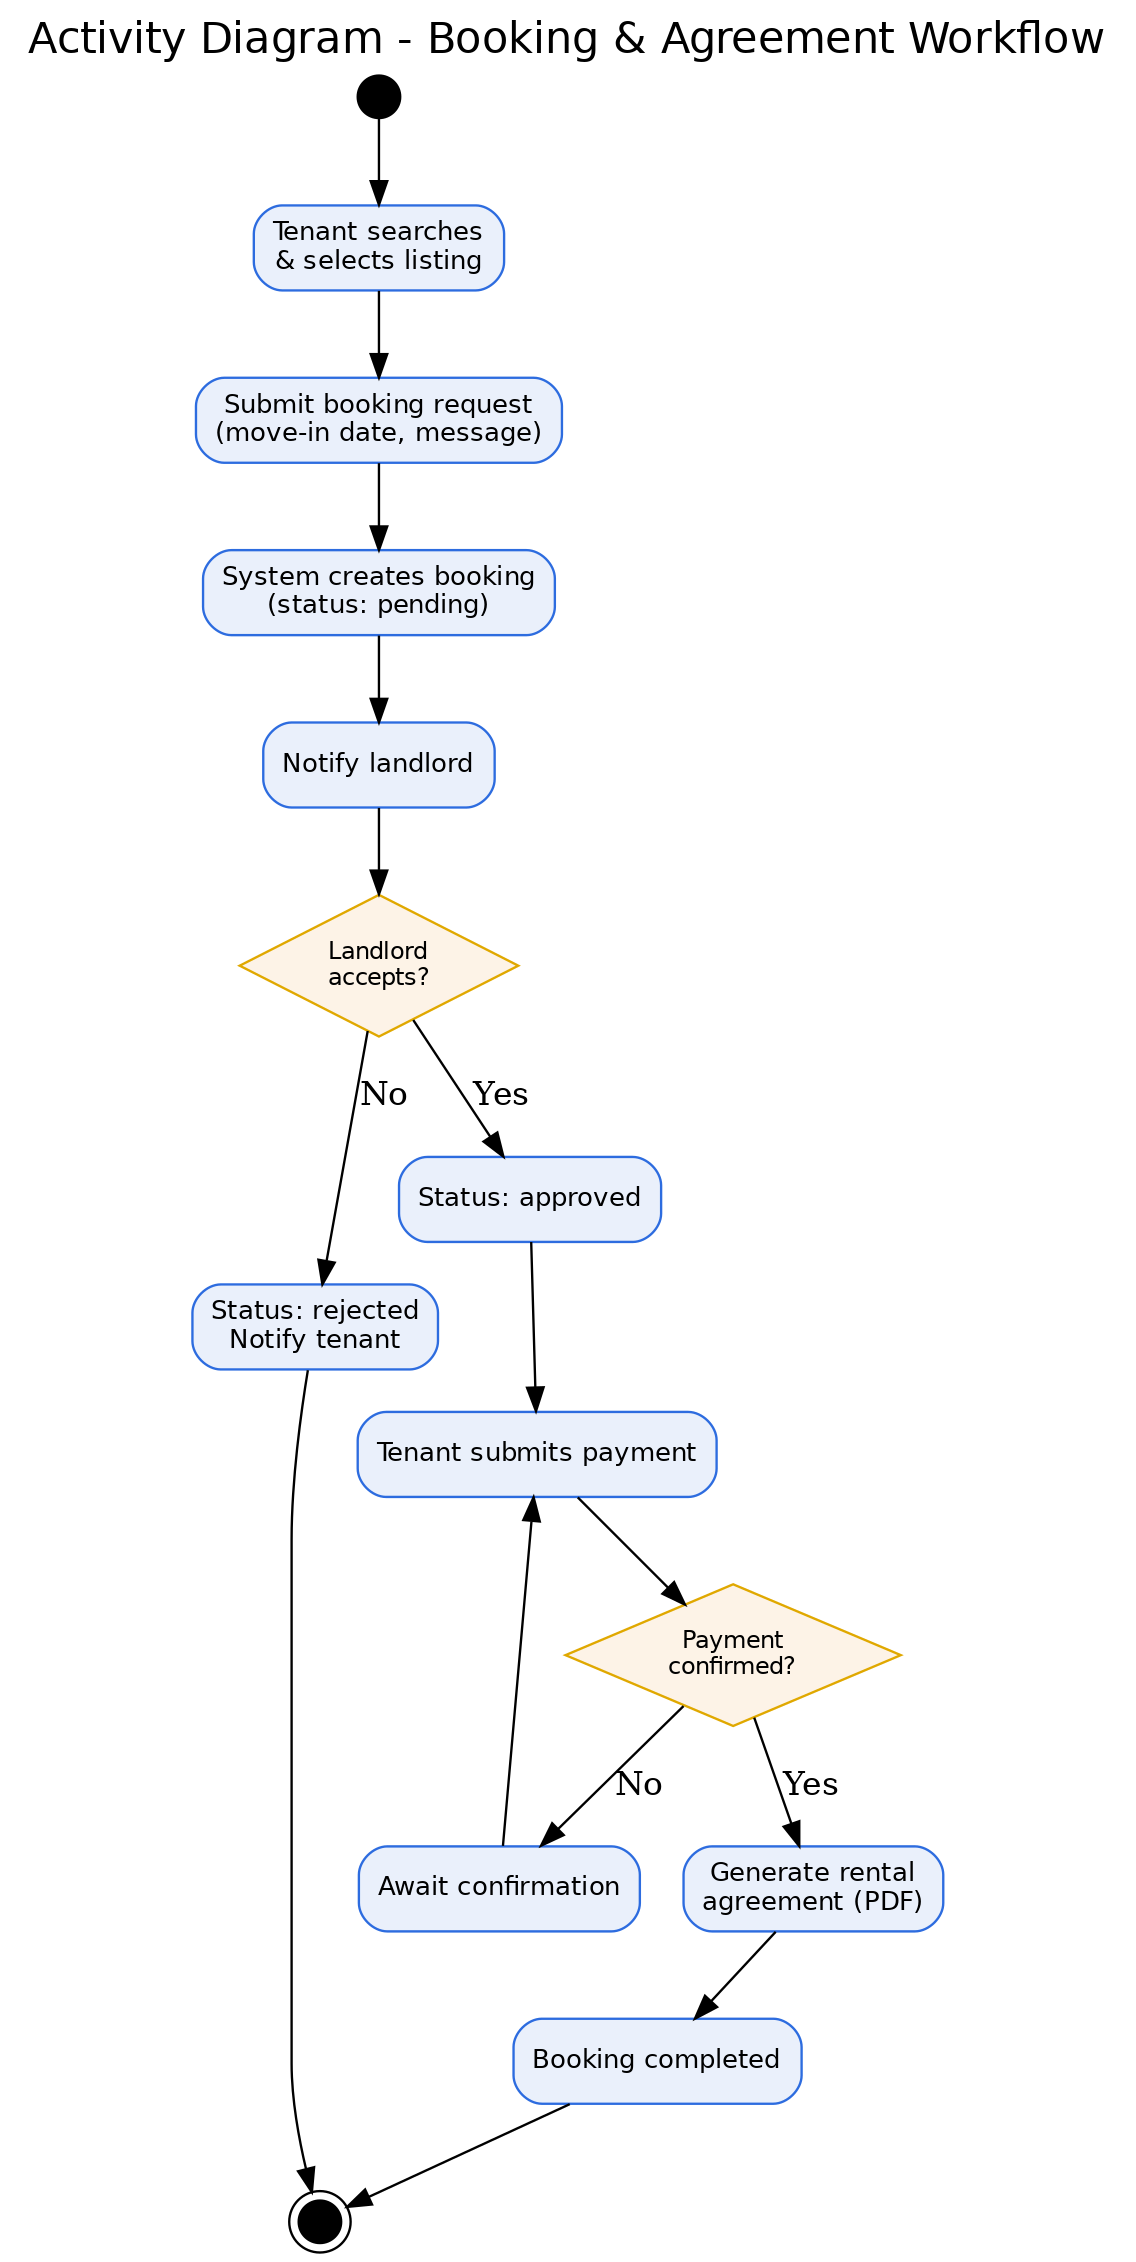
\includegraphics[width=0.67\textwidth]{Figures/Activity Diagram.png}
\caption{Activity Diagram (Sample)}
\label{fig:activity}
\end{figure}

\subsubsection{Module 1: User Management}

This activity diagram illustrates the registration, login, and verification workflow. The flow begins with the user submitting credentials, proceeds through input validation, account creation, and email verification, and includes a decision point where unverified accounts are restricted from protected actions until verification completes.

\subsubsection{Module 2: Property Listing and Booking}

This activity diagram captures the core rental workflow: a landlord creates a listing, the listing awaits verification, a tenant searches and submits a booking request, the landlord accepts or rejects it, payment is recorded, and a digital agreement is generated. Decision nodes handle validation failures, rejected bookings, and unconfirmed payments.

\subsubsection{Module 3: Admin Module}

This activity diagram describes administrator operations, including reviewing verification requests, approving or rejecting documents, managing user status, confirming payments, and viewing analytics.

%%%%%%%%%%%%%%%%%%%%%%%%%%%%%%%%%%%%%%%%%%%%%%%%%%%%%%
\subsection{Class Diagram}

The class diagram shows the static structure of the system, including the principal domain classes, their attributes, and their relationships.

\begin{figure}[h]
\centering
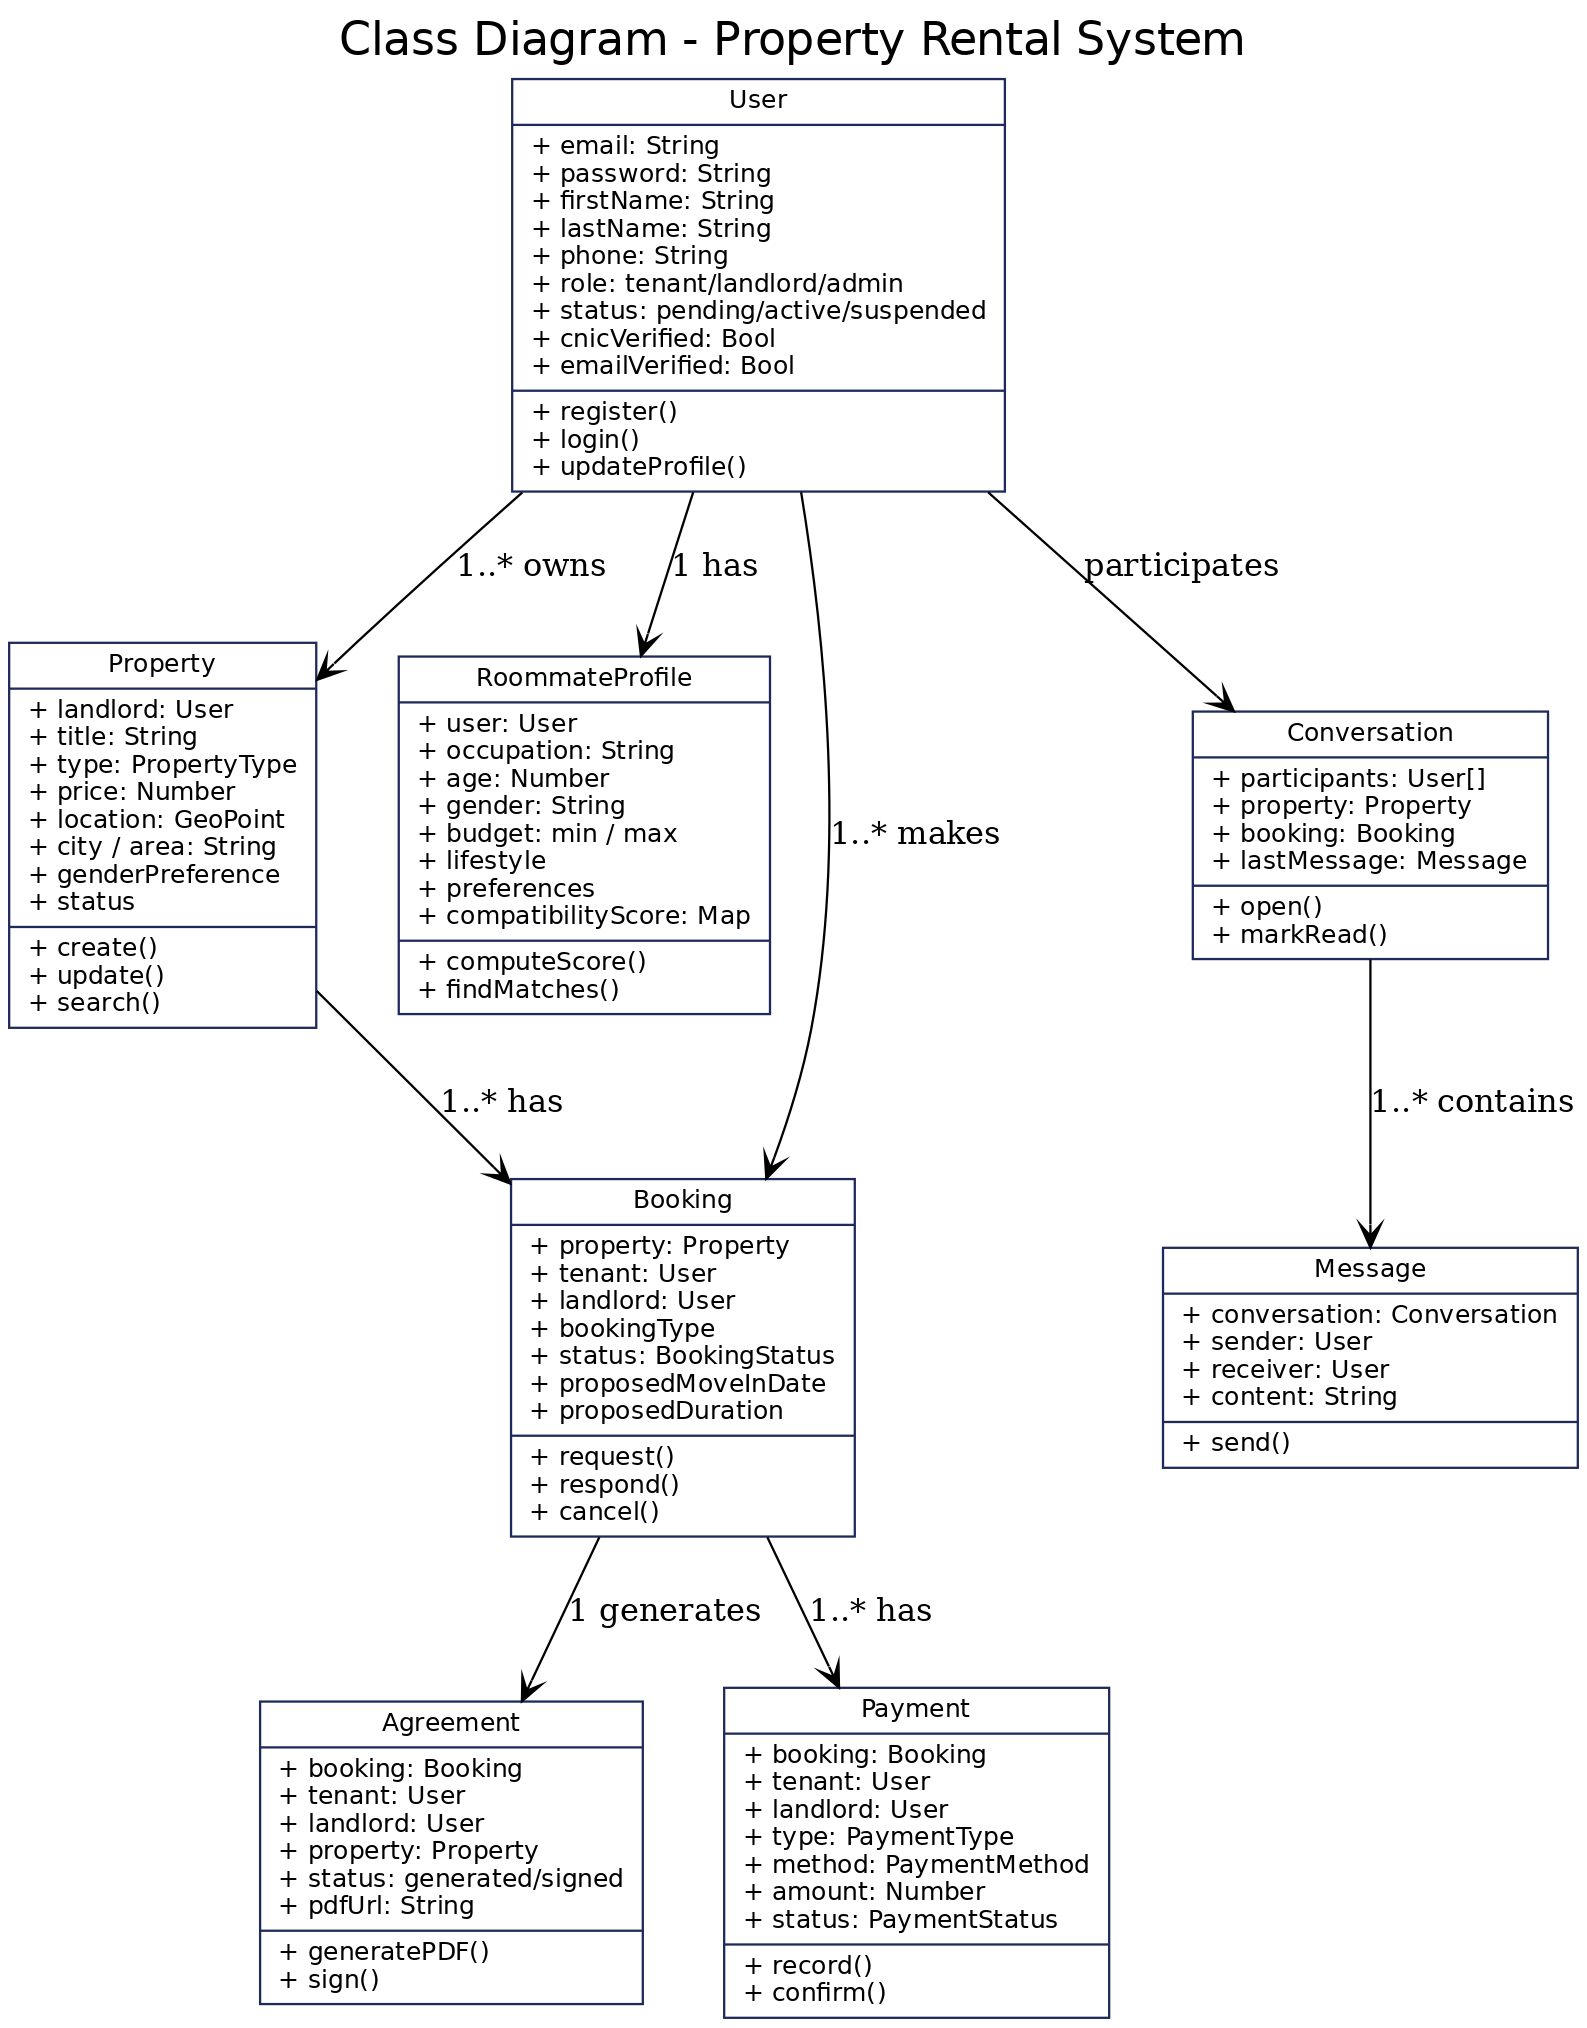
\includegraphics[width=0.88\textwidth]{Figures/Class Diagram.png}
\caption{Class Diagram (Sample)}
\label{fig:class}
\end{figure}

The key classes of Property Rental System are \texttt{User} (with subtypes distinguished by role), \texttt{Property}, \texttt{RoommateProfile}, \texttt{Booking}, \texttt{Agreement}, \texttt{Payment}, \texttt{Conversation}, \texttt{Message}, \texttt{Document}, and \texttt{LandlordBankAccount}. A \texttt{User} acting as a landlord owns many \texttt{Property} listings; a \texttt{User} acting as a tenant creates many \texttt{Booking} records; each \texttt{Booking} relates one tenant, one landlord, and one property and may generate one \texttt{Agreement} and one or more \texttt{Payment} records. \texttt{Conversation} aggregates many \texttt{Message} objects between two users. Each \texttt{User} may have one \texttt{RoommateProfile}, which the matching service uses to compute compatibility. These relationships include association, aggregation, and role-based specialisation.

%%%%%%%%%%%%%%%%%%%%%%%%%%%%%%%%%%%%%%%%%%%%%%%%%%%%%%
\subsection{Sequence Diagrams}

Sequence diagrams show the interaction between objects over time, including the request-response flow between the actor, the system components, and the database.

\subsubsection{Sequence Diagram -- User Login}

\begin{figure}[h]
\centering
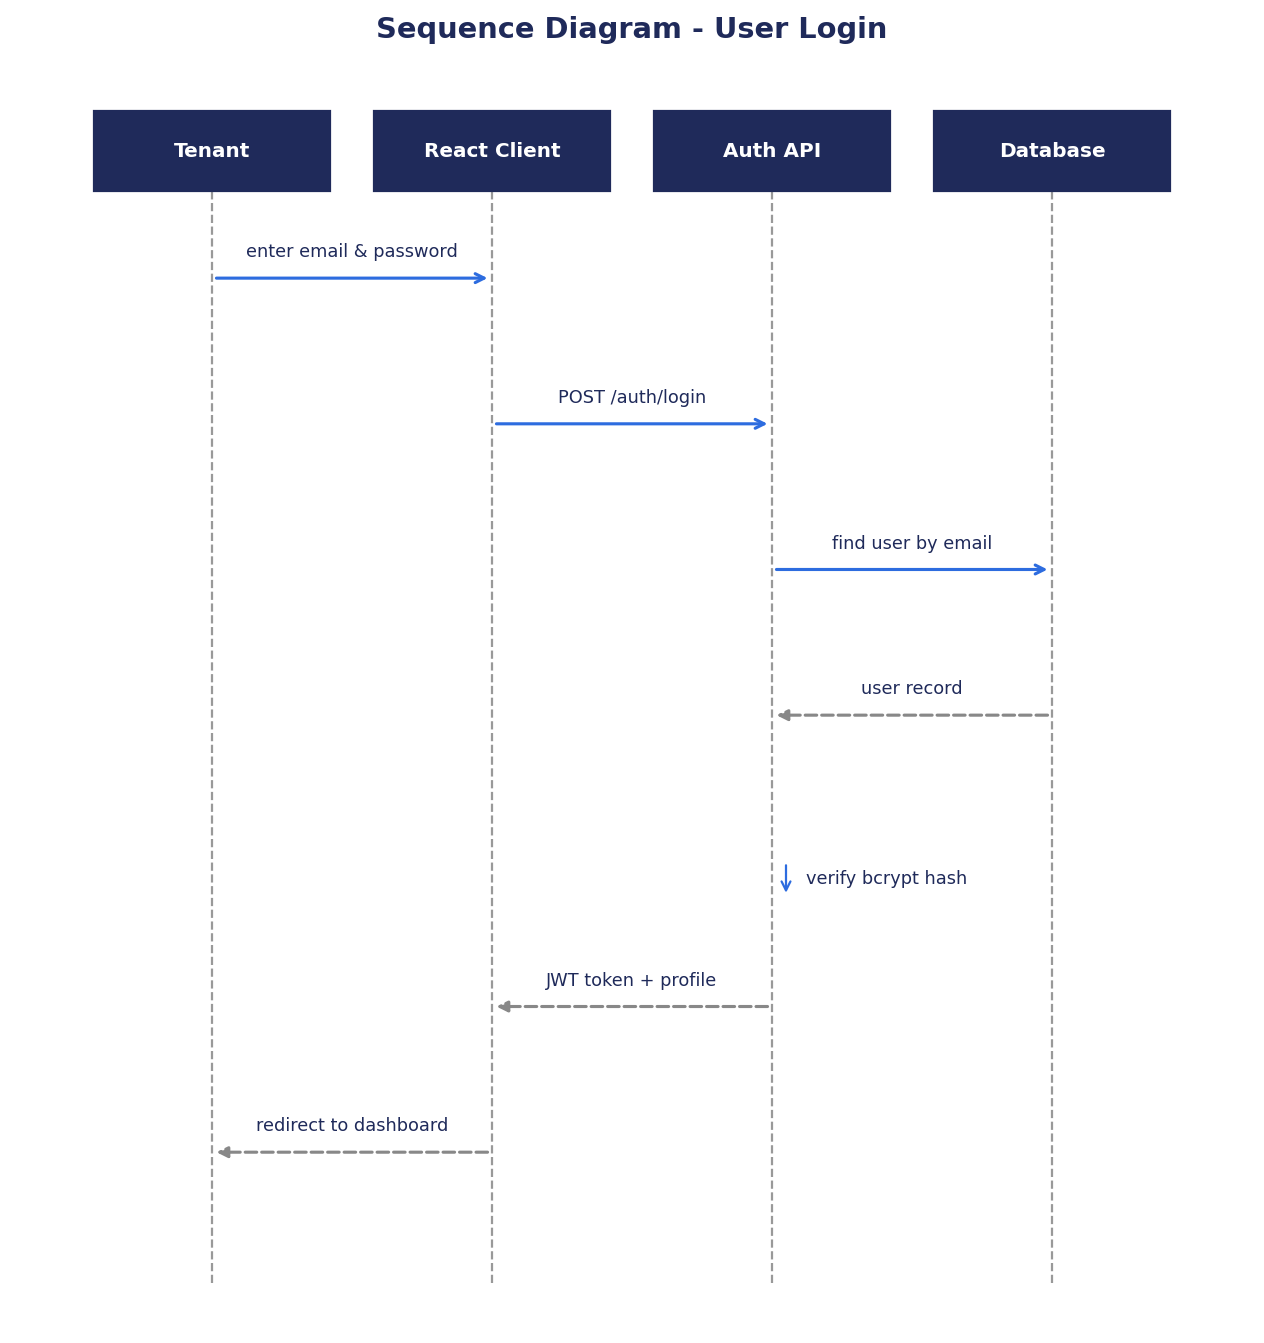
\includegraphics[width=0.8\textwidth]{Figures/Sequence Diagram 2.png}
\caption{Sequence Diagram -- User Login (Sample)}
\label{fig:seq1}
\end{figure}

In the login sequence, the user submits credentials to the React client, which sends them to the authentication endpoint. The authentication service validates the credentials against the user record in MongoDB, verifies the hashed password, issues a JWT on success, and returns it to the client, which stores it for subsequent authenticated requests.

\subsubsection{Sequence Diagram -- Booking and Agreement}

\begin{figure}[h]
\centering
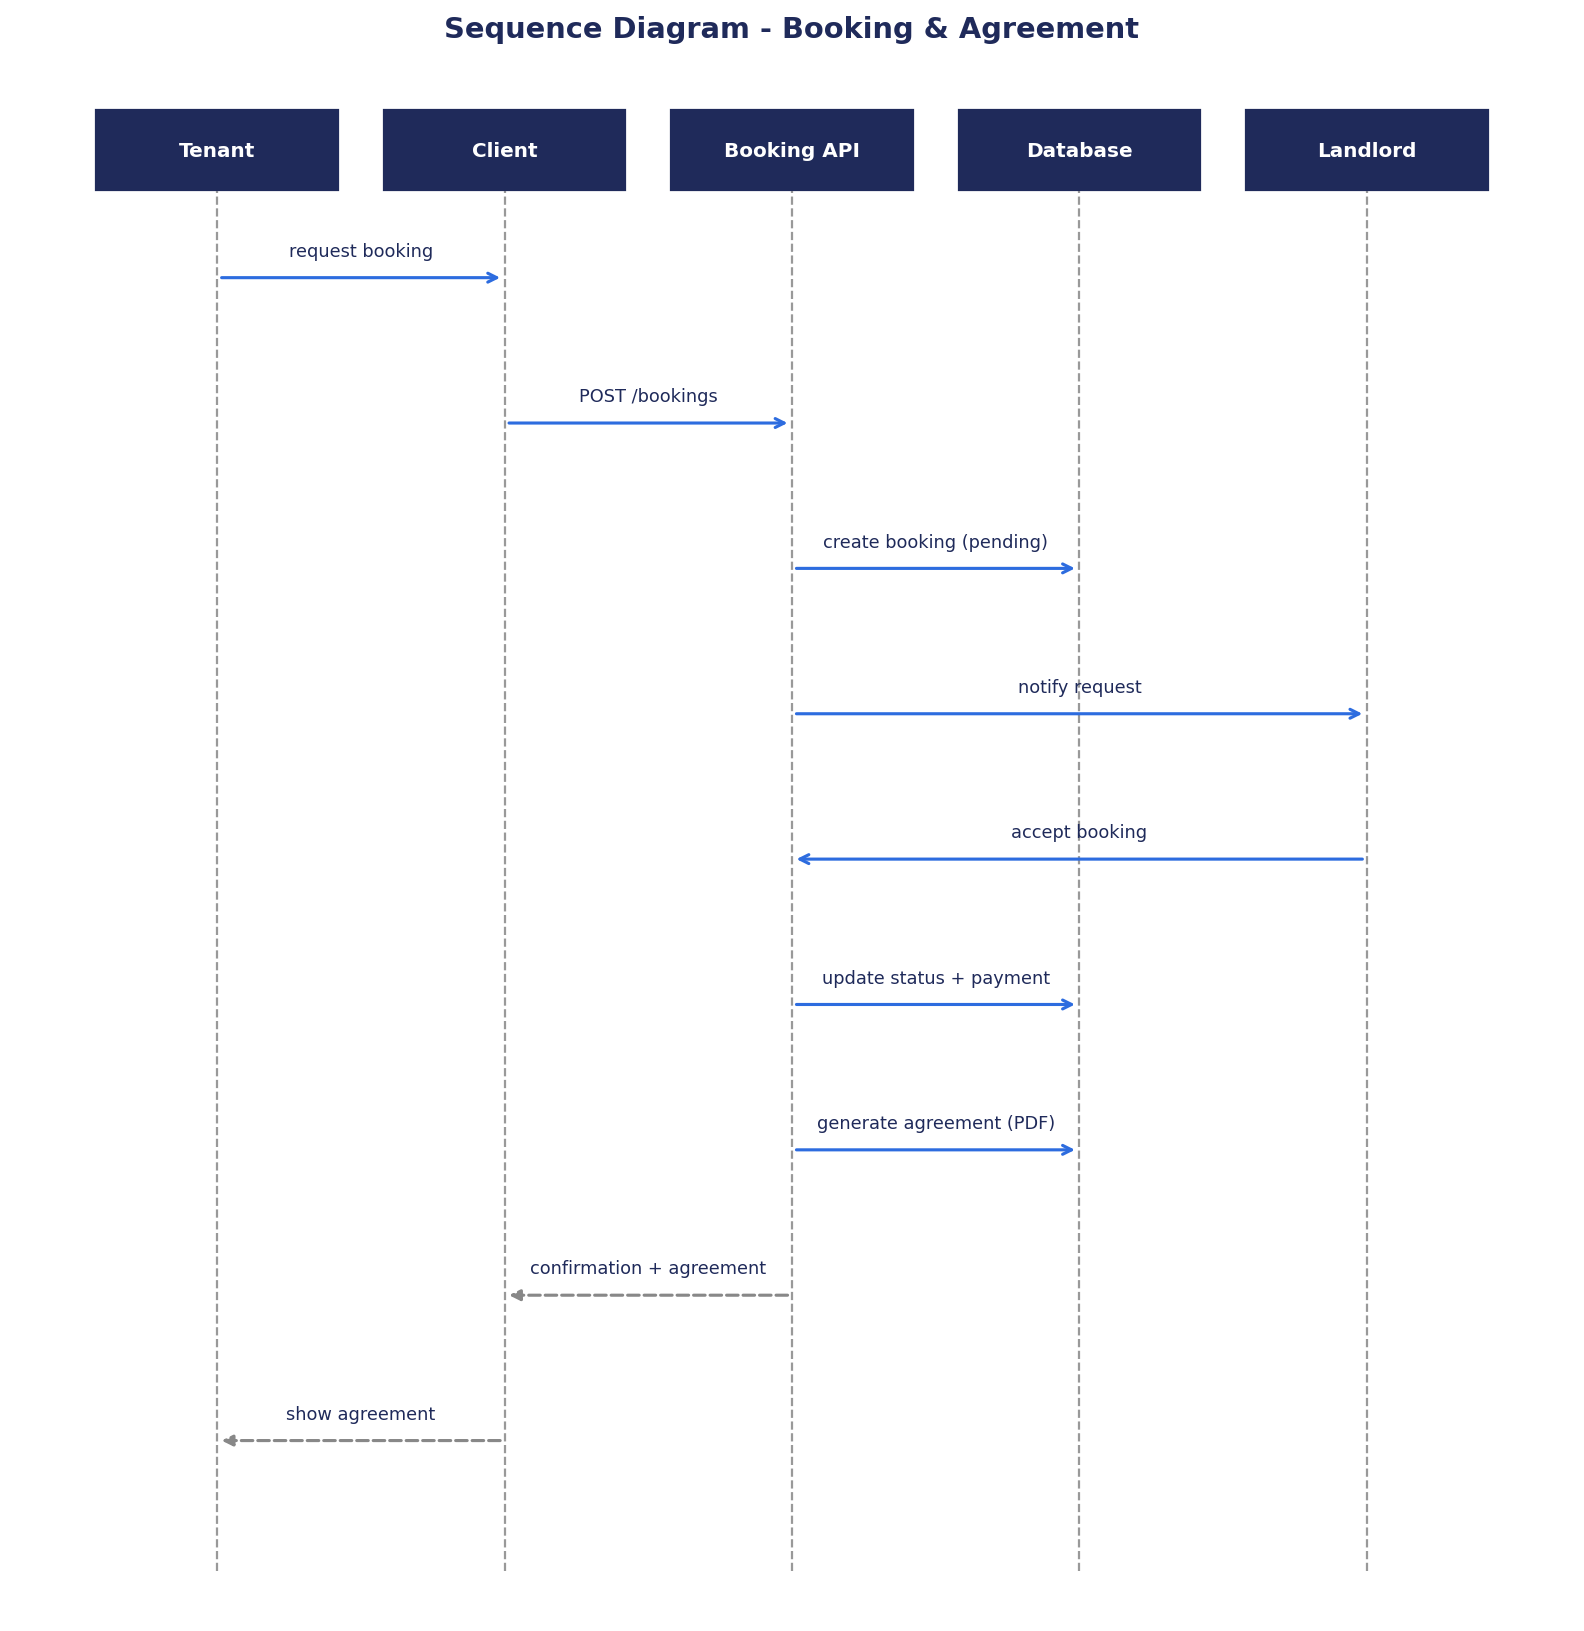
\includegraphics[width=0.8\textwidth]{Figures/Sequence Diagram.png}
\caption{Sequence Diagram -- Booking and Agreement (Sample)}
\label{fig:seq2}
\end{figure}

In the booking sequence, the tenant submits a booking request; the booking service creates a pending booking and notifies the landlord; upon acceptance and confirmed payment, the agreement service generates a PDF rental agreement and persists it, after which both parties are notified.

%%%%%%%%%%%%%%%%%%%%%%%%%%%%%%%%%%%%%%%%%%%%%%%%%%%%%%
\subsection{State Transition Diagrams}

\begin{figure}[h]
\centering
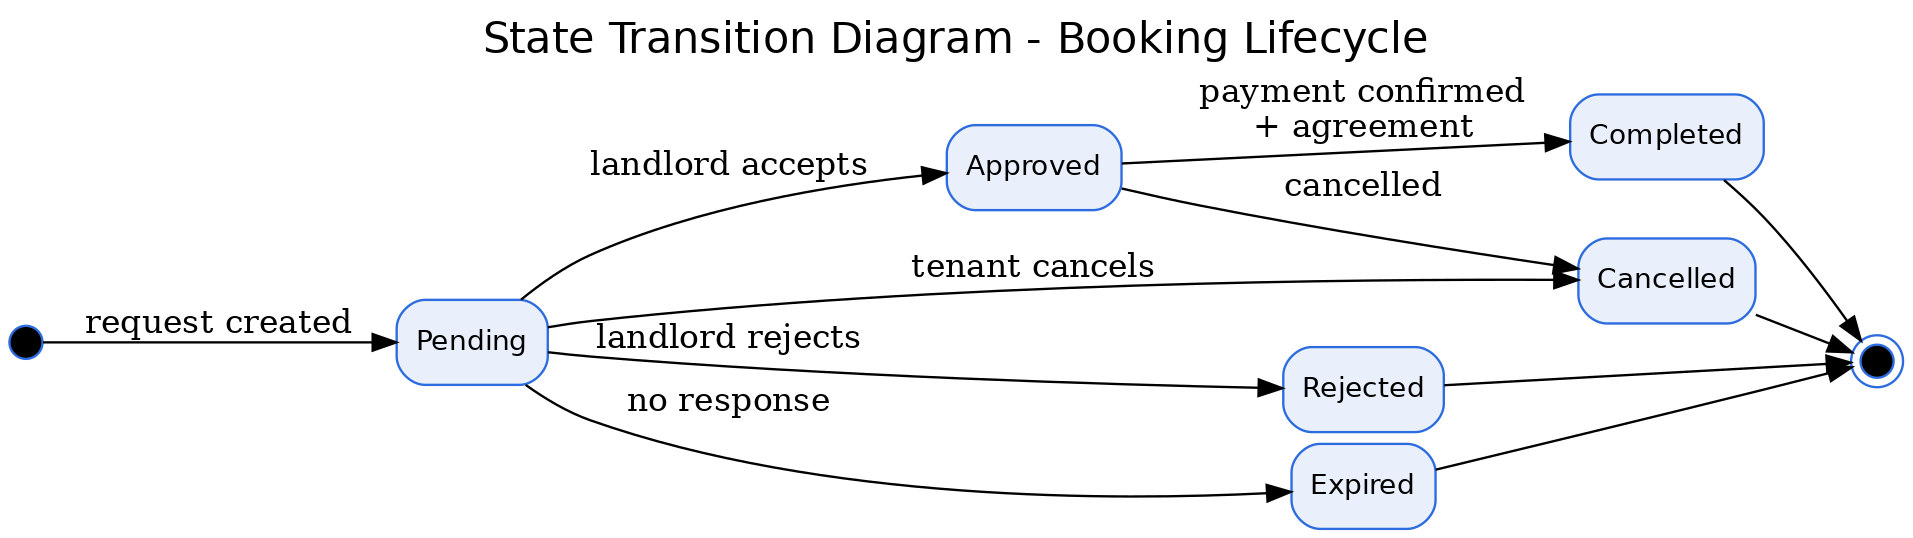
\includegraphics[width=0.77\textwidth]{Figures/State Transition.png}
\caption{State Transition Diagram (Sample)}
\label{fig:state}
\end{figure}

State transition diagrams show how key entities change state over their lifecycle. Two important examples in Property Rental System are the user account and the booking. A \textbf{User account} transitions through the states \textit{Pending} (just registered), \textit{Active} (verified), and \textit{Suspended} (administratively blocked). A \textbf{Booking} transitions through \textit{Pending} (requested), \textit{Accepted} or \textit{Rejected} (landlord decision), \textit{Confirmed} (payment recorded), and \textit{Completed} or \textit{Cancelled}. A \textbf{Property} listing transitions through \textit{Pending Verification}, \textit{Active}, and \textit{Inactive}. Each transition is triggered by a specific event, such as approval, payment, or administrative action.

%%%%%%%%%%%%%%%%%%%%%%%%%%%%%%%%%%%%%%%%%%%%%%%%%%%%%%
\section{Data Flow Diagrams}

Data Flow Diagrams describe how data moves within the system. Different levels provide increasing detail.

\subsection{Level 1 Data Flow Diagram}

\begin{figure}[h]
\centering
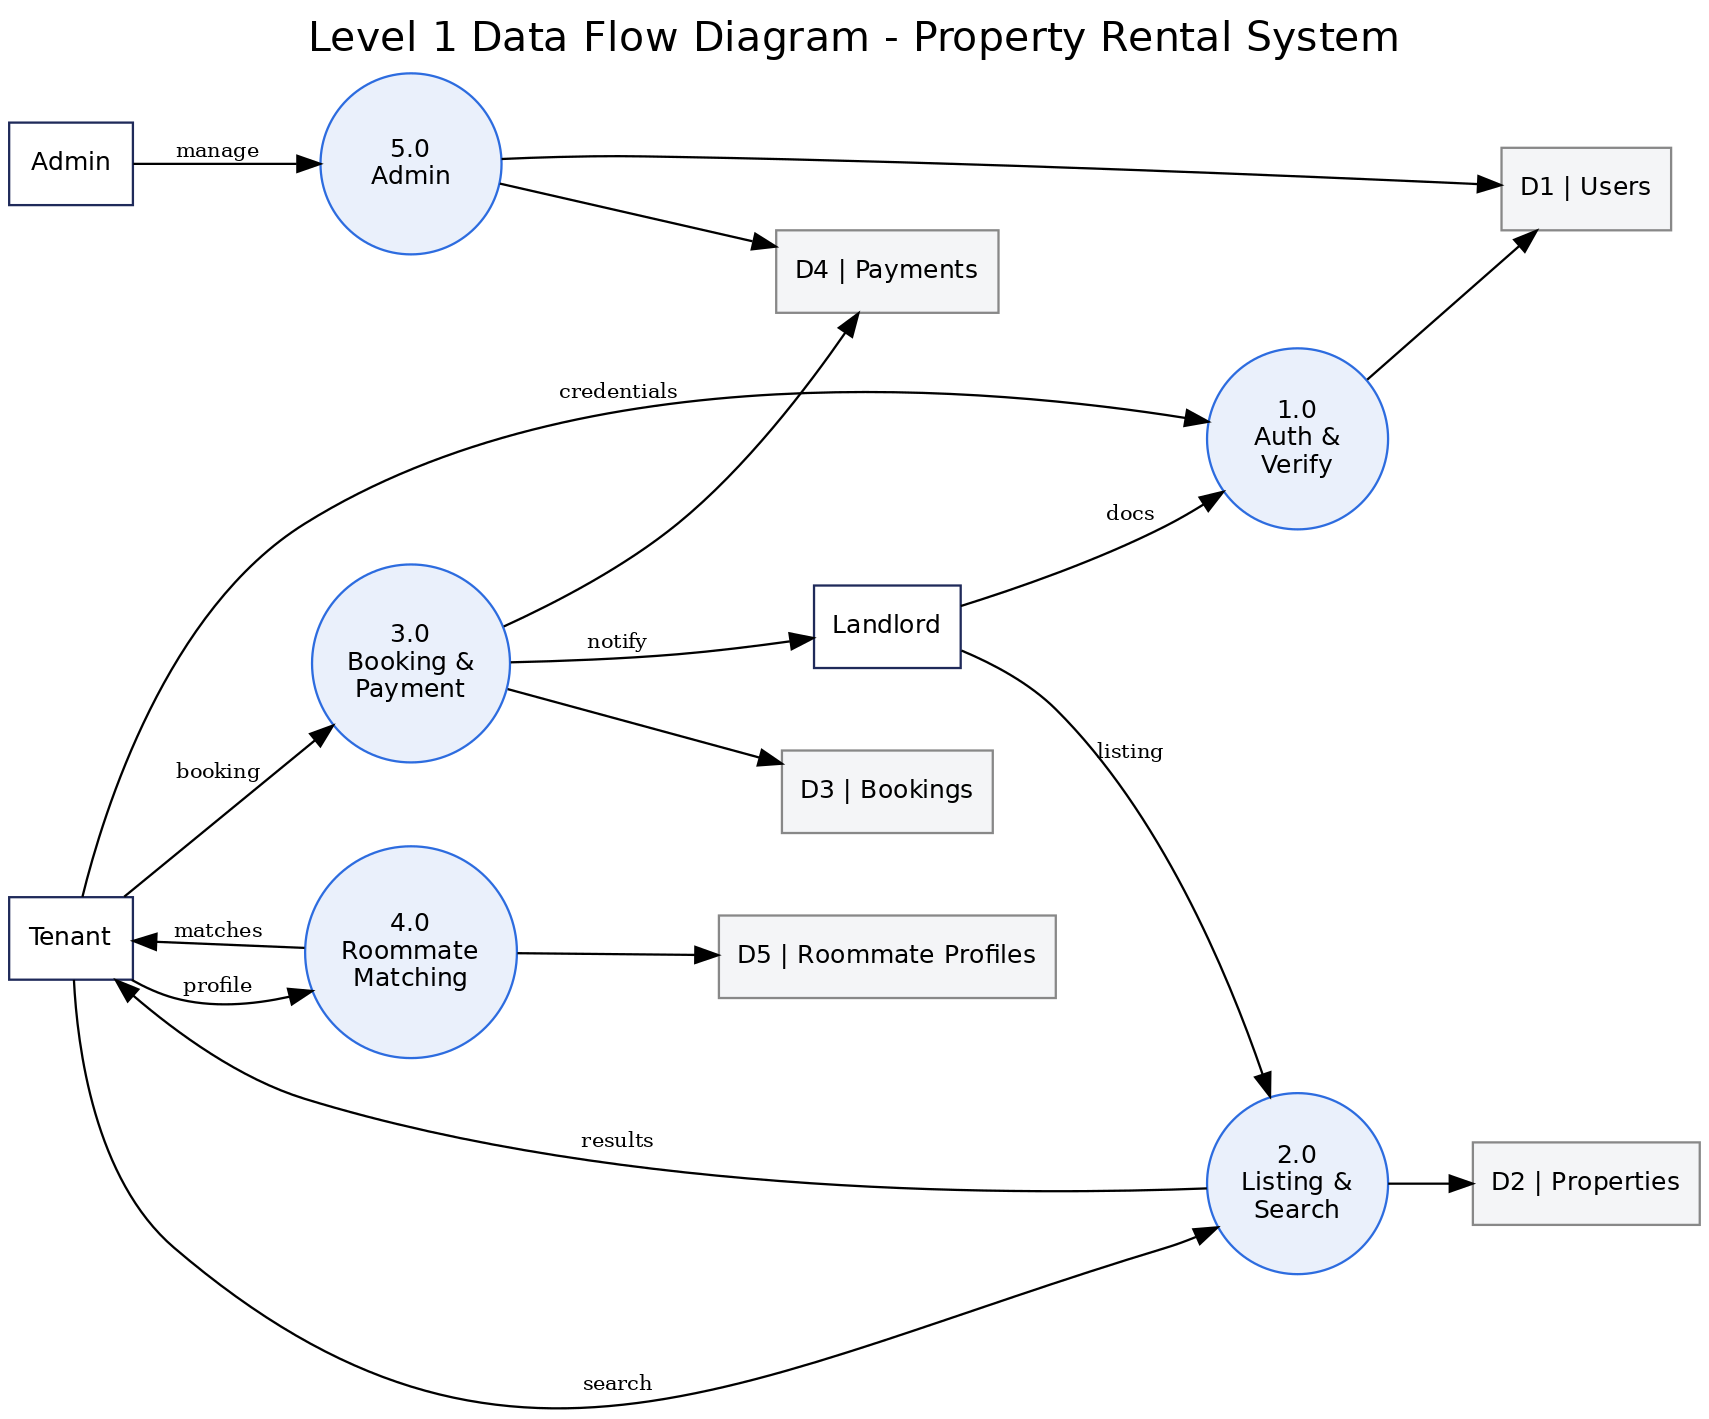
\includegraphics[width=0.9\textwidth]{Figures/DFD Sample.png}
\caption{Level 1 Data Flow Diagram (Sample)}
\label{fig:dfd1}
\end{figure}

The Level 1 DFD decomposes the platform into its major sub-processes: the Authentication and Verification process, the Property Listing and Search process, the Booking and Payment process, the Roommate Matching process, and the Administration process. Each process exchanges data with the relevant data stores, namely the Users, Properties, Bookings, Payments, Agreements, and Roommate Profiles collections, while external entities (tenant, landlord, administrator) provide inputs and receive outputs.

\subsection{Level 2 Data Flow Diagram}

\begin{figure}[h]
\centering
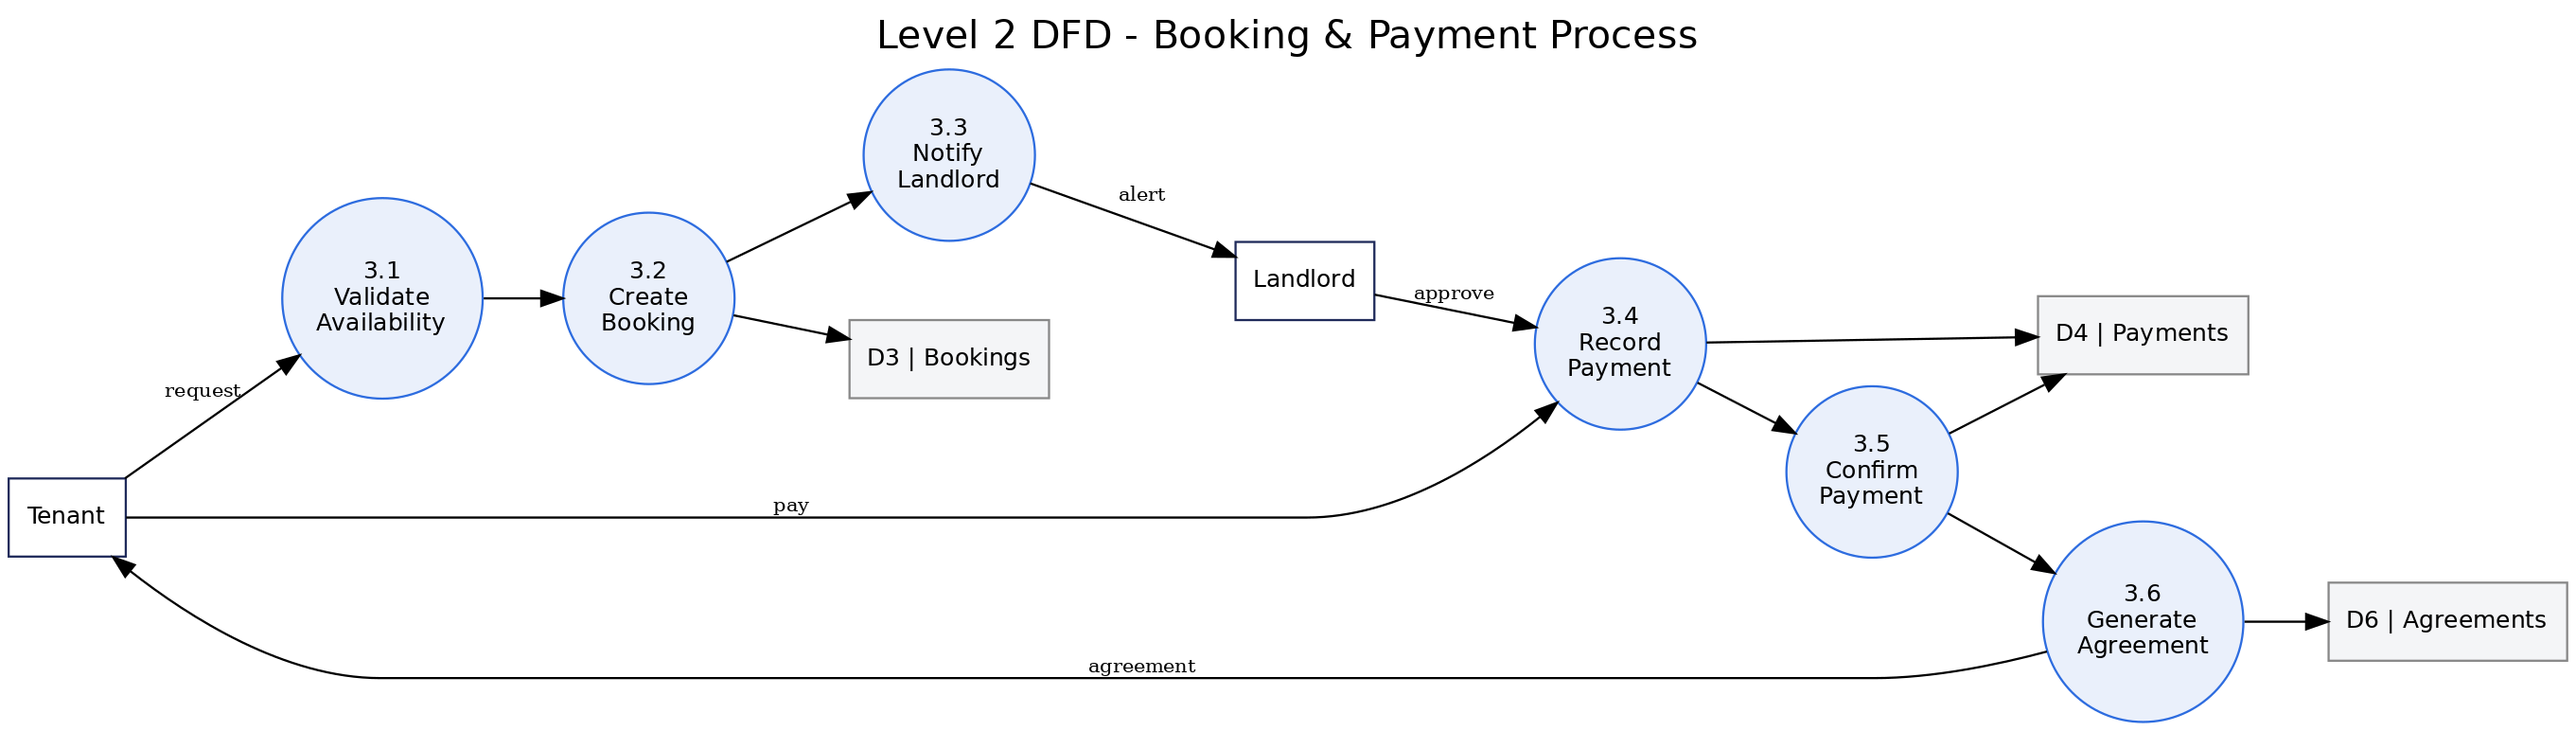
\includegraphics[width=0.9\textwidth]{Figures/DFD Sample 2.png}
\caption{Level 2 Data Flow Diagram (Sample)}
\label{fig:dfd2}
\end{figure}

The Level 2 DFD further decomposes the Booking and Payment process. It details the sub-processes of validating booking availability, creating the booking record, notifying the landlord, recording payment details, confirming payment, and triggering agreement generation, showing the data flowing into and out of the Bookings, Payments, and Agreements data stores at each step.

%%%%%%%%%%%%%%%%%%%%%%%%%%%%%%%%%%%%%%%%%%%%%%%%%%%%%%
\section{Data Design}

This section describes how data is structured, stored, and managed. Property Rental System uses MongoDB, a document-oriented NoSQL database, accessed through the Mongoose object data modelling library. The schema is organised into discrete collections that mirror the domain entities. Documents reference one another by ObjectId to model relationships, and indexes are defined on frequently queried fields, including a 2dsphere geospatial index on property location and compound indexes on status fields, to ensure efficient queries. Security mechanisms include password hashing, role-based access control, and restricted access to verification documents.

%%%%%%%%%%%%%%%%%%%%%%%%%%%%%%%%%%%%%%%%%%%%%%%%%%%%%%
\subsection{Entity Relationship Diagram (ERD)}

\begin{figure}[h]
\centering
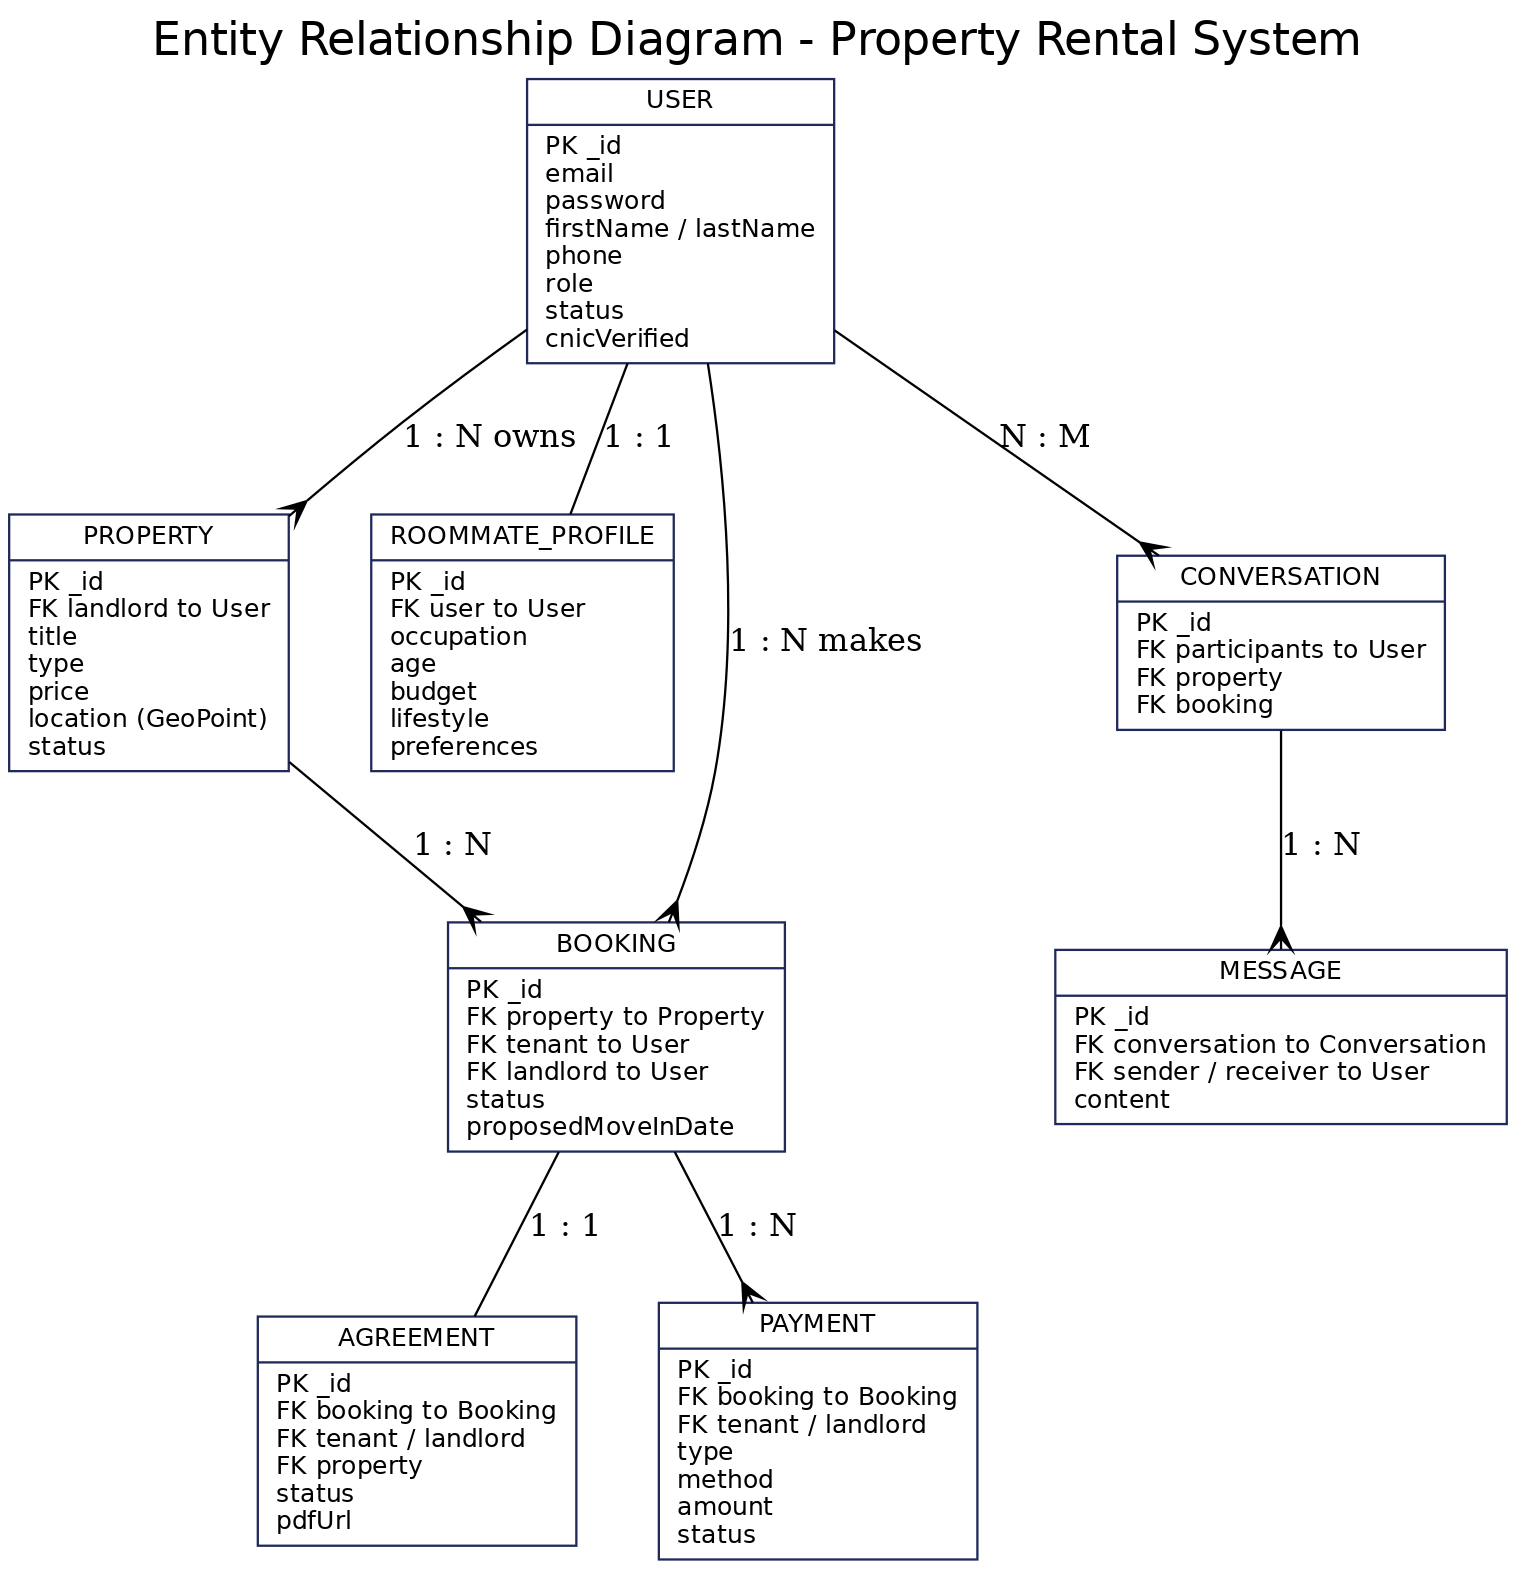
\includegraphics[width=0.9\textwidth]{Figures/ER Diagram.png}
\caption{Entity Relationship Diagram (Sample)}
\label{fig:erd}
\end{figure}

The ERD represents the logical structure of the Property Rental System database. The principal entities are User, Property, RoommateProfile, Booking, Agreement, Payment, Conversation, Message, Document, and LandlordBankAccount. A User (landlord) owns many Properties (1:N); a User (tenant) makes many Bookings (1:N); a Property has many Bookings (1:N); a Booking produces one Agreement (1:1) and one or more Payments (1:N); a Conversation contains many Messages (1:N) and links two Users; and a User has one RoommateProfile (1:1). \textit{(Replace the sample figure with the finalised Property Rental System ERD before submission.)}

%%%%%%%%%%%%%%%%%%%%%%%%%%%%%%%%%%%%%%%%%%%%%%%%%%%%%%
\subsection{Database Architecture}

Property Rental System uses a client-server database architecture in which the Express application server is the sole client of the MongoDB database. Property images and verification documents are stored in cloud media storage, with the database retaining only their secure references. This separation keeps the database lean and allows media to be served efficiently. The design supports cloud deployment and can be scaled through MongoDB replication and sharding if required.

%%%%%%%%%%%%%%%%%%%%%%%%%%%%%%%%%%%%%%%%%%%%%%%%%%%%%%
\section{Database Schema Diagram}

\begin{figure}[h]
\centering
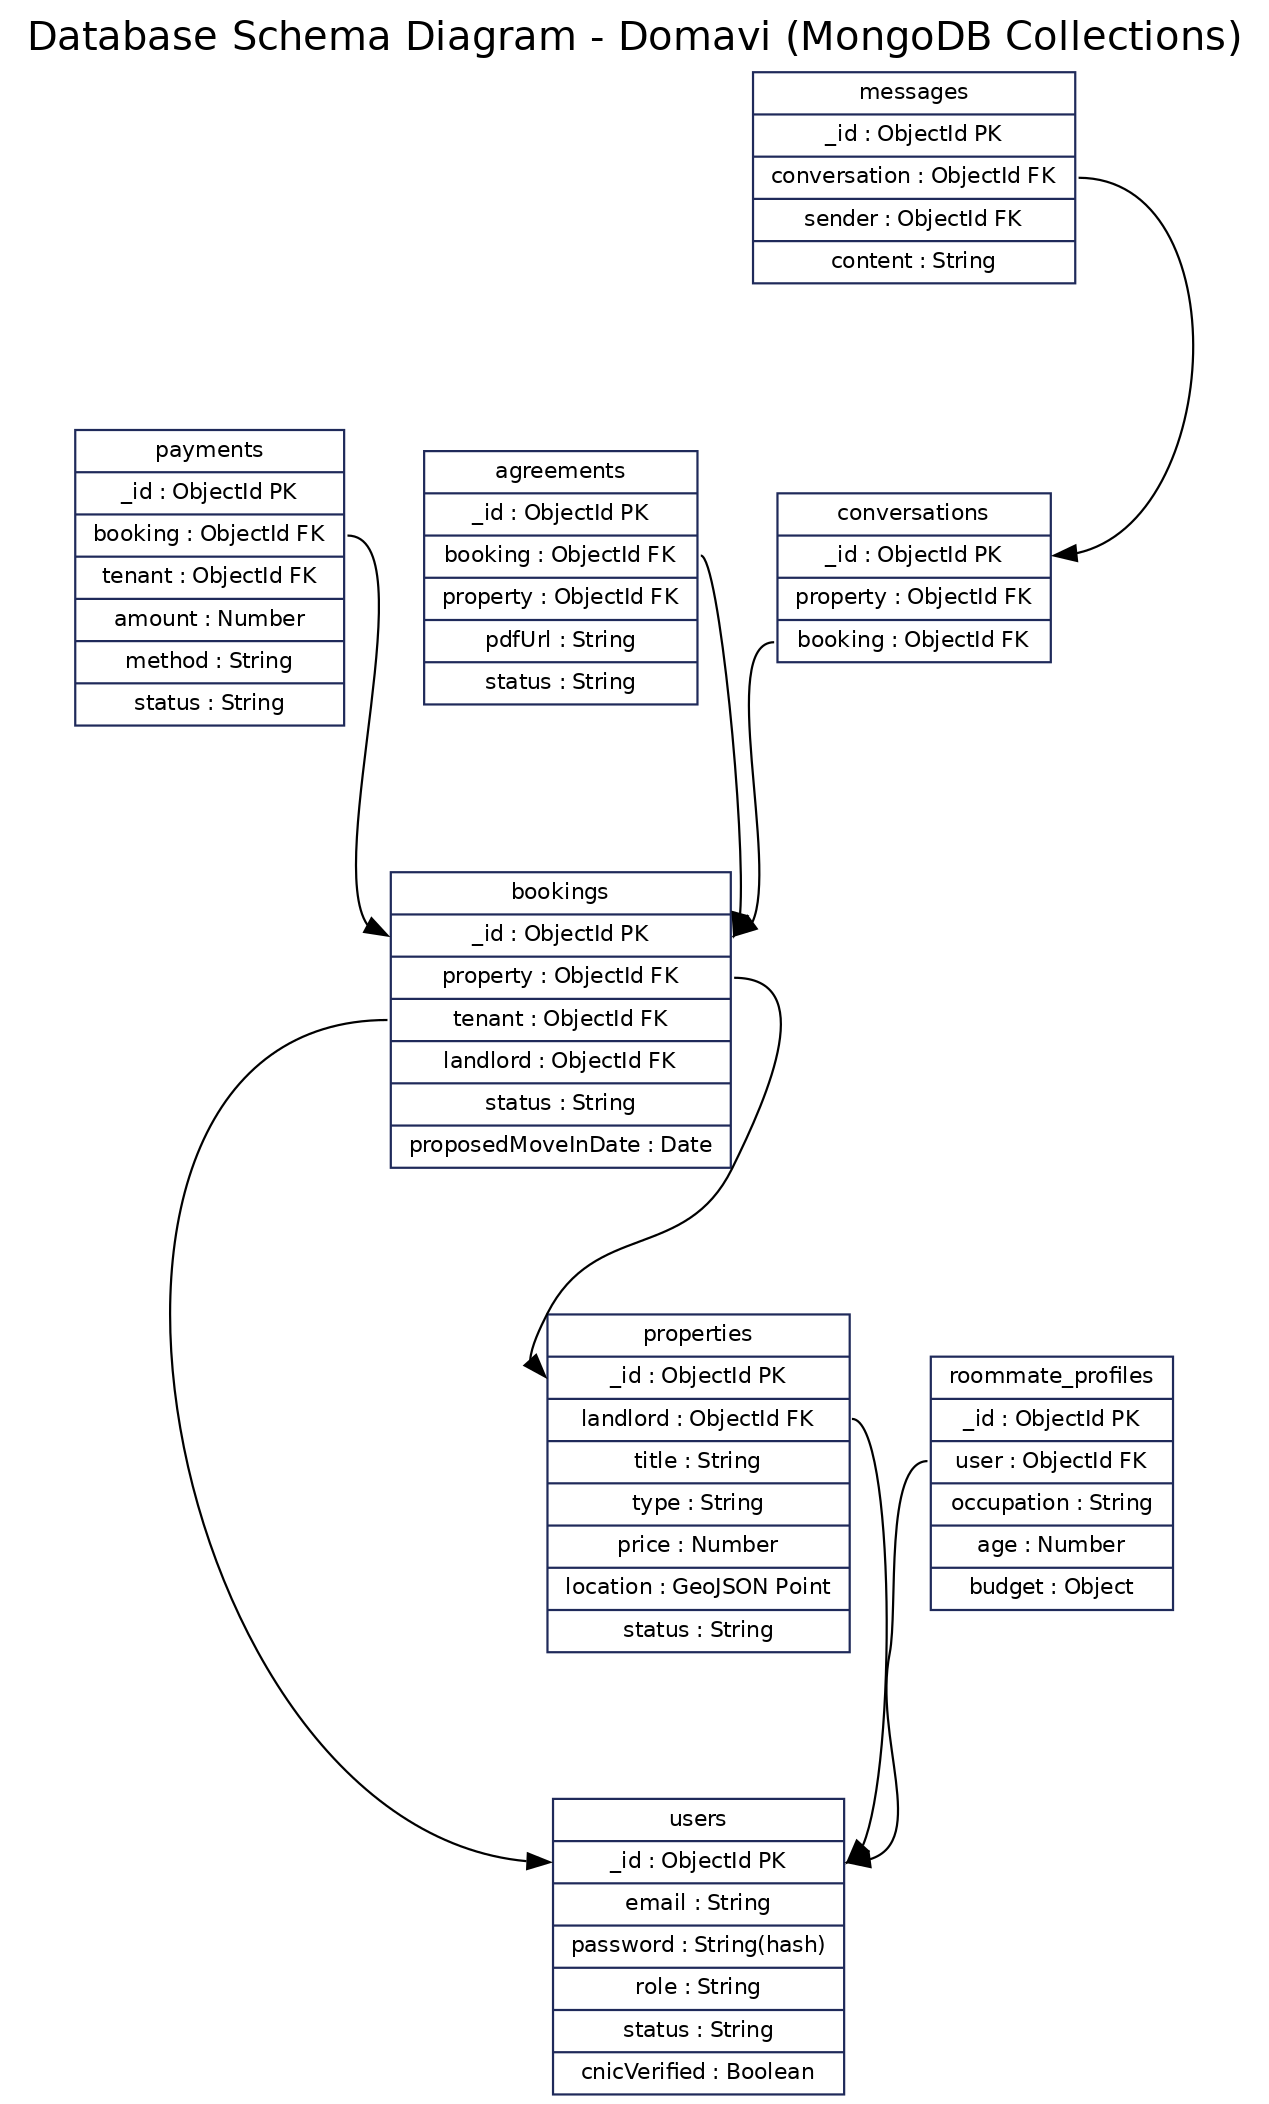
\includegraphics[width=0.9\textwidth]{Figures/Database Diagram.png}
\caption{Database Schema Diagram (Sample)}
\label{fig:dbschema}
\end{figure}

The schema diagram represents the physical structure of the collections, including field names, types, and the reference relationships between collections. The design supports data integrity through schema validation in Mongoose, efficient querying through indexing, scalability through a document model that avoids costly joins, and security through controlled access to sensitive fields. \textit{(Replace the sample figure with the finalised Property Rental System schema diagram.)}

%%%%%%%%%%%%%%%%%%%%%%%%%%%%%%%%%%%%%%%%%%%%%%%%%%%%%%
\subsection{Data Dictionary}

The data dictionary defines the structure of the principal data elements of the User collection as a representative example.

\begin{table}[h]
\centering
\caption{Data Dictionary -- User Collection}
\begin{tabularx}{\textwidth}{|p{3cm}|p{2.5cm}|X|}
\hline
\textbf{Field Name} & \textbf{Type} & \textbf{Description} \\
\hline
\_id & ObjectId & Unique identifier for each user \\
\hline
name & String & Full name of the user \\
\hline
email & String & Unique registered email address \\
\hline
passwordHash & String & Securely hashed password \\
\hline
role & String & User role: tenant, landlord, or admin \\
\hline
status & String & Account status: pending, active, or suspended \\
\hline
isVerified & Boolean & Indicates whether identity verification is complete \\
\hline
createdAt & Date & Account creation timestamp \\
\hline
\end{tabularx}
\end{table}

%%%%%%%%%%%%%%%%%%%%%%%%%%%%%%%%%%%%%%%%%%%%%%%%%%%%%%
%===========================================================
\section{Database Collections}
%===========================================================

This section describes the logical database design of Property Rental System. As a NoSQL system, the database is organised into collections, each modelling a domain entity with primary identifiers, references, and major attributes. The design ensures data consistency, integrity, security, and scalability.

%%%%%%%%%%%%%%%%%%%%%%%%%%%%%%%%%%%%%%%%%%%%%%%%%%%%%%
\subsection{User Collection}
%%%%%%%%%%%%%%%%%%%%%%%%%%%%%%%%%%%%%%%%%%%%%%%%%%%%%%

The User collection stores authentication credentials and profile information for all roles and supports role-based access control and secure authentication.

\begin{table}[h]
\centering
\caption{User Collection Structure}

\begin{tabularx}{\textwidth}{|p{3cm}|p{3cm}|p{3cm}|X|}
\hline
\textbf{Field Name} & \textbf{Data Type} & \textbf{Constraint} & \textbf{Description} \\
\hline
\_id & ObjectId & Primary Key & Unique identifier \\
\hline
name & String & Not Null & User's full name \\
\hline
email & String & Unique, Not Null & Login email address \\
\hline
passwordHash & String & Not Null & Hashed password \\
\hline
role & String & Not Null & tenant / landlord / admin \\
\hline
status & String & Default pending & Account status \\
\hline
createdAt & Date & Default now & Creation timestamp \\
\hline
\end{tabularx}

\end{table}

%%%%%%%%%%%%%%%%%%%%%%%%%%%%%%%%%%%%%%%%%%%%%%%%%%%%%%
\subsection{Property Collection}
%%%%%%%%%%%%%%%%%%%%%%%%%%%%%%%%%%%%%%%%%%%%%%%%%%%%%%

The Property collection stores micro-rental listings created by landlords, including location as a GeoJSON point to support geospatial search.

\begin{table}[h]
\centering
\caption{Property Collection Structure}

\begin{tabularx}{\textwidth}{|p{3cm}|p{3cm}|p{3cm}|X|}
\hline
\textbf{Field Name} & \textbf{Data Type} & \textbf{Constraint} & \textbf{Description} \\
\hline
\_id & ObjectId & Primary Key & Unique identifier \\
\hline
landlord & ObjectId & Foreign Key (User) & Owner of the listing \\
\hline
title & String & Not Null & Listing title \\
\hline
type & String & Not Null & room / bed space / hostel \\
\hline
price & Number & Not Null & Rent amount \\
\hline
location & GeoJSON Point & 2dsphere index & Geographic coordinates \\
\hline
status & String & Default pending\_verification & Listing status \\
\hline
\end{tabularx}

\end{table}

%%%%%%%%%%%%%%%%%%%%%%%%%%%%%%%%%%%%%%%%%%%%%%%%%%%%%%
\subsection{Booking, Payment, and Agreement Collections}
%%%%%%%%%%%%%%%%%%%%%%%%%%%%%%%%%%%%%%%%%%%%%%%%%%%%%%

The \textbf{Booking} collection records each rental request, referencing the tenant, landlord, and property, and tracking the booking status and move-in date. The \textbf{Payment} collection records payment type, method, amount, bank details, and status (pending or confirmed), referencing the related booking, tenant, and landlord. The \textbf{Agreement} collection stores the auto-generated rental agreement reference and terms for a confirmed booking. The \textbf{RoommateProfile} collection stores each user's lifestyle, preferences, budget, location, and schedule data along with cached compatibility scores. The \textbf{Conversation} and \textbf{Message} collections store in-app messaging, while \textbf{Document} and \textbf{LandlordBankAccount} store verification documents and landlord payout details respectively.

%%%%%%%%%%%%%%%%%%%%%%%%%%%%%%%%%%%%%%%%%%%%%%%%%%%%%%
\subsection{Relationships Between Collections}
%%%%%%%%%%%%%%%%%%%%%%%%%%%%%%%%%%%%%%%%%%%%%%%%%%%%%%

\begin{itemize}
    \item \textbf{One-to-One (1:1):} Each user has one roommate profile; each confirmed booking has one agreement.
    \item \textbf{One-to-Many (1:N):} A landlord owns many properties; a tenant makes many bookings; a property has many bookings; a conversation has many messages.
    \item \textbf{Many-to-Many (M:N):} Tenants interact with many properties through bookings and conversations, and properties are viewed by many tenants, resolved through the Booking and Conversation collections.
\end{itemize}

%%%%%%%%%%%%%%%%%%%%%%%%%%%%%%%%%%%%%%%%%%%%%%%%%%%%%%
\subsection{Security and Data Integrity}
%%%%%%%%%%%%%%%%%%%%%%%%%%%%%%%%%%%%%%%%%%%%%%%%%%%%%%

\begin{itemize}
    \item Password hashing using a secure algorithm (bcrypt) with salting.
    \item Role-based access control (RBAC) enforced through authentication middleware.
    \item Schema-level validation and constraints enforced by Mongoose.
    \item Secure communication over HTTPS and authenticated API requests via JWT.
    \item Restricted access to verification documents and regular database backups.
\end{itemize}

%%%%%%%%%%%%%%%%%%%%%%%%%%%%%%%%%%%%%%%%%%%%%%%%%%%%%%
\subsection{Scalability Considerations}
%%%%%%%%%%%%%%%%%%%%%%%%%%%%%%%%%%%%%%%%%%%%%%%%%%%%%%

\begin{itemize}
    \item Indexing on frequently queried attributes, including a geospatial index for location-based search.
    \item A document data model that avoids expensive joins and supports horizontal scaling.
    \item Offloading of media to cloud storage to keep the database lightweight.
    \item Support for MongoDB replication and sharding for future growth.
\end{itemize}

%%%%%%%%%%%%%%%%%%%%%%%%%%%%%%%%%%%%%%%%%%%%%%%%%%%%%%
\section{Chapter Summary}
%%%%%%%%%%%%%%%%%%%%%%%%%%%%%%%%%%%%%%%%%%%%%%%%%%%%%%

This chapter presented the comprehensive software design of the Property Rental System platform.
It justified an object-oriented, layered MVC design methodology and an Agile
process model, and described the system through a context diagram and a
three-layer client-server architecture. Detailed UML models, including activity,
class, sequence, and state transition diagrams, were developed to describe the
system's behaviour and structure, and data flow diagrams illustrated internal
data movement. The chapter further elaborated the database design through the
entity relationship model, schema diagram, data dictionary, and collection
specifications, addressing relationships, security, integrity, and scalability.
Overall, this chapter establishes a clear technical blueprint that guides the
implementation phase discussed in the next chapter.

% ============================================
% Chapter 5 – Implementation
% ============================================

\chapter{Implementation}

This chapter describes the practical implementation of the Property Rental System platform. It explains how the design presented in Chapter~4 was translated into working modules, algorithms, user interfaces, and integrated services using the MERN technology stack.

% -------------------------------------------------
% 5.1 Development Environment
% -------------------------------------------------

\section{Development Environment}

The platform was developed using a modern JavaScript and TypeScript toolchain. The development environment is summarised below.

\begin{itemize}
    \item \textbf{IDE / Editor:} Visual Studio Code with ESLint and Prettier for linting and formatting.
    \item \textbf{Languages:} TypeScript across both the frontend and backend, with HTML and CSS in the presentation layer.
    \item \textbf{Frontend Framework:} React with the Vite build tool, Tailwind CSS for styling, and Zustand for state management.
    \item \textbf{Backend Framework:} Node.js with Express.js, organised into routes, controllers, services, and middleware.
    \item \textbf{Database:} MongoDB with the Mongoose object data modelling library.
    \item \textbf{Version Control:} Git with a GitHub repository for collaboration between the two team members.
    \item \textbf{Operating System:} Cross-platform development on Windows and macOS.
    \item \textbf{Hardware:} Standard development laptops with 8--16 GB RAM; no specialised GPU is required.
\end{itemize}

% -------------------------------------------------
% 5.2 Core Module Implementation
% -------------------------------------------------

\section{Core Module Implementation}

Each major module of Property Rental System was implemented as a cohesive set of routes, a controller, and a service class on the backend, with corresponding pages and components on the frontend.

\subsection{Module 1: Authentication and Verification}

This module implements registration, login, email verification, and password reset. The authentication service hashes passwords with bcrypt, issues JSON Web Tokens on successful login, and exposes middleware that validates tokens and enforces role-based access control. The verification service manages the upload of CNIC and ownership documents to cloud storage and records verification requests for administrative review.

\subsection{Module 2: Property Listing and Search}

The property service handles the creation, update, retrieval, and removal of listings. Each property stores its location as a GeoJSON point, and a 2dsphere index enables commute-based proximity queries. The search functionality combines geospatial filtering with attribute filters for price, room type, and gender preference, returning only active and verified listings to tenants.

\subsection{Module 3: Booking, Payment, and Agreement}

The booking service manages the lifecycle of a booking from pending request to acceptance, confirmation, and completion. The payment service records payment details and bank information and updates the payment status upon administrative confirmation. Once a booking is confirmed, the agreement service generates a digital rental agreement as a PDF and stores its reference against the booking.

\subsection{Module 4: Roommate Matching}

The roommate matching module is implemented in a dedicated matcher service that computes a weighted compatibility score between roommate profiles. Profiles capture lifestyle, preferences, budget, location, and schedule attributes. The service computes a score per category, applies category weights, aggregates them into an overall score, caches results to avoid recomputation, and returns a ranked list of top matches.

\subsection{Module 5: Messaging and Administration}

The chat service manages conversations and messages between tenants and landlords. The administration module provides endpoints for reviewing verification requests, managing user accounts and status, overseeing payments, and retrieving analytics, all protected by an admin-only access guard.

% -------------------------------------------------
% 5.3 Algorithm Implementation
% -------------------------------------------------

\section{Algorithm Implementation}

The most significant algorithm in Property Rental System is the roommate compatibility matching algorithm. It quantifies how well two users would live together by comparing their lifestyle profiles across five weighted categories and producing an overall compatibility score on a scale of 0 to 100.

\subsection{Algorithm: Weighted Roommate Compatibility Scoring}

\textbf{Input:} Two roommate profiles, $P_1$ and $P_2$ \\
\textbf{Output:} Overall compatibility score $S \in [0, 100]$

The algorithm evaluates five categories with the following default weights: lifestyle (0.25), preferences (0.25), budget (0.20), location (0.15), and schedule (0.15). For each category it computes a normalised similarity score between the two profiles, multiplies it by the category weight, and sums the weighted scores to obtain the overall result. To find matches for a given user, the algorithm computes this score against all candidate profiles and returns the highest-scoring candidates.

\textbf{Step-by-Step Working:}

\begin{enumerate}
    \item Retrieve the requesting user's roommate profile.
    \item For each candidate profile:
    \begin{itemize}
        \item Compute the lifestyle similarity score.
        \item Compute the preferences similarity score.
        \item Compute the budget similarity score.
        \item Compute the location similarity score.
        \item Compute the schedule similarity score.
        \item Multiply each category score by its weight and sum to obtain the overall score.
        \item Cache the overall score for reuse.
    \end{itemize}
    \item Sort candidates in descending order of overall score.
    \item Return the top N candidates as matches.
\end{enumerate}

\textbf{Pseudo Code:}

\begin{verbatim}
Algorithm RoommateMatch(P_user, Candidates, Weights):
1. matches = []
2. For each C in Candidates:
      lifestyle  = similarity(P_user.lifestyle,   C.lifestyle)
      prefs      = similarity(P_user.preferences, C.preferences)
      budget     = similarity(P_user.budget,      C.budget)
      location   = similarity(P_user.location,    C.location)
      schedule   = similarity(P_user.schedule,    C.schedule)
      score = lifestyle*0.25 + prefs*0.25 + budget*0.20
              + location*0.15 + schedule*0.15
      matches.add({ candidate: C, score: round(score) })
3. Sort matches by score descending
4. Return top N matches
\end{verbatim}

\textbf{Explanation:} The weighted approach allows the most behaviourally significant factors, lifestyle and preferences, to influence the result most strongly, while still accounting for budget, location, and schedule. Caching previously computed scores reduces repeated computation when the same pair is evaluated again. The algorithm integrates with the backend and is triggered when a tenant opens the roommate matches page.

% -------------------------------------------------
% 5.4 External APIs / SDKs
% -------------------------------------------------

\section{External APIs / SDKs}

Property Rental System integrates several third-party services to deliver its features.

\begin{table}[h]
\centering
\caption{External APIs and Services Used}
\begin{tabularx}{\textwidth}{|p{3.2cm}|X|p{3.5cm}|}
\hline
\textbf{API / Service} & \textbf{Purpose} & \textbf{Used In Module} \\
\hline
Google Maps API & Geocoding of addresses, proximity-based search, and map display with location pins. & Property Search \\
\hline
Cloud Media Storage & Secure storage and delivery of property images and verification documents. & Property, Verification \\
\hline
SMTP Email Service & Email verification and event notifications. & Authentication, Notifications \\
\hline
\end{tabularx}
\end{table}

% -------------------------------------------------
% 5.5 User Interface Implementation
% -------------------------------------------------

\section{User Interface Implementation}

This section presents the major user interface screens of Property Rental System. Each screen is described in terms of its purpose, components, interaction flow, backend integration, and validation. Students should include screenshots of each major screen in the final report.

\subsection{UI Design Approach}

The Property Rental System interface follows a clean, minimalistic design built with Tailwind CSS and a component library organised using the atomic design methodology, in which small atoms (buttons, inputs, badges) compose into molecules (property cards, search bars, filter chips) and organisms (complete sections). A consistent colour scheme, typography, and spacing scale are defined as design tokens to ensure visual consistency. The layout follows a mobile-first, responsive strategy so that the application adapts smoothly from mobile to desktop, and accessibility considerations such as readable font sizes and clear focus states are applied throughout.

\subsection{Screen-wise Implementation}

\subsubsection{Screen 1: Authentication Screen}

\textbf{Purpose:} Allows tenants and landlords to register and log in. \\
\textbf{Components:} Email field, password field, role selector, login and sign-up buttons, and a forgot-password link. \\
\textbf{Functional Flow:} On submission, the client validates the inputs and calls the authentication API; on success a token is stored and the user is redirected to their role-specific dashboard. \\
\textbf{Backend Integration:} Calls the authentication endpoints; the server validates credentials and returns a JWT. \\
\textbf{Validation:} Required-field, email-format, and password-strength validation with clear inline error messages.

\subsubsection{Screen 2: Search and Listings Screen}

\textbf{Purpose:} Enables tenants to discover accommodation near a chosen location. \\
\textbf{Components:} Location input, filter controls (price, type, gender preference), a results list of property cards, and an interactive map. \\
\textbf{Functional Flow:} Entering a location triggers a geospatial search; results update in both the list and the map. \\
\textbf{Backend Integration:} Calls the property search endpoint with location and filter parameters. \\
\textbf{Validation:} Graceful empty-state handling when no listings match.

\subsubsection{Screen 3: Add Property Screen}

\textbf{Purpose:} Allows verified landlords to create a new listing. \\
\textbf{Components:} Form fields for title, description, type, price, amenities, location picker, and image upload. \\
\textbf{Functional Flow:} The landlord completes the form and submits; the listing is created with pending-verification status. \\
\textbf{Backend Integration:} Calls the property creation endpoint and uploads images to cloud storage. \\
\textbf{Validation:} Required fields, valid price, and at least one image.

\subsubsection{Screen 4: Roommate Matches Screen}

\textbf{Purpose:} Displays a ranked list of compatible roommates. \\
\textbf{Components:} Compatibility cards showing the candidate and their match score. \\
\textbf{Functional Flow:} On load, the system computes and displays the top matches for the user's profile. \\
\textbf{Backend Integration:} Calls the matching endpoint. \\
\textbf{Security Considerations:} Only accessible to authenticated tenants with a completed profile.

\subsubsection{Screen 5: Admin Dashboard Screen}

\textbf{Purpose:} Provides administrators with oversight of the platform. \\
\textbf{Components:} Navigation, summary data cards, verification queue, user management table, payment oversight, and analytics charts. \\
\textbf{Functional Flow:} Data loads dynamically from administrative endpoints. \\
\textbf{Backend Integration:} Calls admin-only endpoints. \\
\textbf{Security Considerations:} Protected by role-based access control restricting access to administrators.

\subsection{Navigation Flow Diagram}

A navigation flow diagram should be included to show how the major screens, the authentication, search, property detail, booking, payments, messages, roommate matches, and admin screens, are connected and how users move between them according to their role. \textit{(Insert the finalised navigation flow diagram in the final report.)}

%%%%%%%%%%%%%%%%%%%%%%%%%%%%%%%%%%%%%%%%%%%%%%%%%%%%%%
\section{Chapter Summary}
%%%%%%%%%%%%%%%%%%%%%%%%%%%%%%%%%%%%%%%%%%%%%%%%%%%%%%

This chapter described the implementation of the Property Rental System platform using the MERN
stack and TypeScript. It outlined the development environment, detailed the
implementation of each core module, and presented the weighted roommate
compatibility algorithm together with its pseudo code. The external APIs for
mapping, media storage, and email were documented, and the major user interface
screens were described in terms of their purpose, components, flow, integration,
and validation. The next chapter presents the testing and evaluation of the
implemented system.

% ============================================
% Chapter 6 – Testing and Evaluation
% ============================================

\chapter{Testing and Evaluation}

This chapter presents the testing strategies and evaluation procedures used to verify the correctness, reliability, and performance of the Property Rental System platform. Testing ensures that all functional and non-functional requirements defined in earlier chapters are satisfied. As Property Rental System is a web application, the evaluation focuses on unit, integration, system, performance, security, and user acceptance testing.

% -------------------------------------------------
% 6.1 Testing Strategy
% -------------------------------------------------

\section{Testing Strategy}

Property Rental System was tested using a combination of automated and manual approaches applied throughout the Agile development cycle. Automated unit tests were written for backend services and controllers using the Jest testing framework, allowing individual functions such as authentication, booking creation, payment recording, and compatibility scoring to be verified in isolation. Integration testing validated the interaction between the React frontend, the Express REST API, and the MongoDB database, with API endpoints exercised to confirm correct request handling, authorisation, and data persistence. System testing was performed manually by walking through complete user journeys for each role, while performance and security testing assessed responsiveness and the robustness of authentication and access control. This layered strategy, moving from the smallest units up to the full system and finally to real users, ensured that defects were caught early and that the platform met its specified requirements.

% -------------------------------------------------
% 6.2 Unit Testing
% -------------------------------------------------

\section{Unit Testing}

Unit testing verified individual functions and modules independently. Each major backend service was tested with valid and invalid inputs, and the expected output and pass/fail status were recorded.

\subsection{UT-01: User Registration and Login}

\begin{table}[h]
\centering
\caption{Unit Test Cases – Authentication}
\begin{tabularx}{\textwidth}{|c|X|X|c|}
\hline
\textbf{Test ID} & \textbf{Input} & \textbf{Expected Output} & \textbf{Result} \\
\hline
UT-01 & Valid registration details & Account created with pending status & Pass \\
\hline
UT-02 & Missing or invalid email & Validation error displayed & Pass \\
\hline
UT-03 & Correct login credentials & JWT issued and access granted & Pass \\
\hline
UT-04 & Incorrect password & Access denied with error & Pass \\
\hline
\end{tabularx}
\end{table}

\subsection{UT-02: Roommate Compatibility Scoring}

\begin{table}[h]
\centering
\caption{Unit Test Cases – Roommate Matching}
\begin{tabularx}{\textwidth}{|c|X|X|c|}
\hline
\textbf{Test ID} & \textbf{Input} & \textbf{Expected Output} & \textbf{Result} \\
\hline
UT-05 & Two identical profiles & Compatibility score near 100 & Pass \\
\hline
UT-06 & Two opposite profiles & Low compatibility score & Pass \\
\hline
UT-07 & List of candidates & Ranked matches sorted by score & Pass \\
\hline
\end{tabularx}
\end{table}

% -------------------------------------------------
% 6.3 Integration Testing
% -------------------------------------------------

\section{Integration Testing}

Integration testing ensured that the platform's modules interact correctly, focusing on communication between the frontend and backend, the correct handling of authenticated API requests, and reliable database persistence. Key cross-module flows such as creating a listing and then searching for it, and submitting a booking and then recording a payment, were validated end to end.

\begin{table}[h]
\centering
\caption{Integration Testing Summary}
\begin{tabularx}{\textwidth}{|c|X|X|c|}
\hline
\textbf{Test ID} & \textbf{Modules Integrated} & \textbf{Expected Result} & \textbf{Result} \\
\hline
IT-01 & Frontend + Backend API & Data retrieved and rendered correctly & Pass \\
\hline
IT-02 & Backend + Database & Records stored and retrieved correctly & Pass \\
\hline
IT-03 & Property + Maps API & Geospatial search returns nearby listings & Pass \\
\hline
IT-04 & Booking + Payment + Agreement & Confirmed booking generates agreement & Pass \\
\hline
\end{tabularx}
\end{table}

% -------------------------------------------------
% 6.4 System Testing
% -------------------------------------------------

\section{System Testing}

System testing validated the complete application workflow for each user role. The tenant journey, registering, searching, viewing a property, messaging a landlord, submitting a booking, making a payment, and receiving an agreement, was tested end to end, as were the landlord journey of verification, listing, and booking management, and the administrator journey of verification review, user management, and analytics. Edge cases such as searches with no results, rejected bookings, unconfirmed payments, and access attempts to unauthorised resources were tested to confirm correct error handling and graceful degradation.

% -------------------------------------------------
% 6.5 Performance Testing
% -------------------------------------------------

\section{Performance Testing}

Performance testing measured the responsiveness of key operations under normal conditions. Page loads and search results were observed to render within the target of approximately three seconds, and indexed geospatial queries returned results quickly. The indicative metrics below summarise observed performance during testing.

\begin{table}[h]
\centering
\caption{Performance Metrics}
\begin{tabularx}{\textwidth}{|c|X|c|}
\hline
\textbf{Metric} & \textbf{Description} & \textbf{Value} \\
\hline
Response Time & Average API response time & $\approx$ 220 ms \\
\hline
Search Latency & Geospatial search response time & $<$ 1 s \\
\hline
Dashboard Load & Time to render main dashboard & $<$ 3 s \\
\hline
\end{tabularx}
\end{table}

% -------------------------------------------------
% 6.6 Security Testing
% -------------------------------------------------

\section{Security Testing}

Security testing focused on authentication, authorisation, and data protection. Authentication was verified by confirming that protected endpoints reject requests without a valid JWT. Authorisation was tested by confirming that role-based access control prevents tenants from accessing landlord or administrator functions and vice versa. Password storage was checked to ensure that only salted bcrypt hashes are persisted, never plaintext passwords. Input handling was tested against malformed and malicious inputs, and the use of parameterised Mongoose queries mitigates injection risks. Communication over HTTPS and restricted access to verification documents were also verified.

% -------------------------------------------------
% 6.7 User Acceptance Testing (UAT)
% -------------------------------------------------

\section{User Acceptance Testing}

User acceptance testing was conducted with a small group of representative users, primarily students, who performed realistic tasks such as searching for a room, viewing roommate matches, and submitting a booking request. Feedback was generally positive, confirming that the platform addresses a real need, and the suggestions gathered were used to refine the interface and performance.

\begin{table}[h]
\centering
\caption{User Feedback Summary}
\begin{tabularx}{\textwidth}{|X|X|}
\hline
\textbf{Feedback} & \textbf{Action Taken} \\
\hline
Navigation could be simpler & Navigation and menus simplified \\
\hline
Search felt slightly slow on first load & Queries and indexes optimised \\
\hline
Wanted clearer match explanations & Compatibility scores made more visible \\
\hline
\end{tabularx}
\end{table}

% -------------------------------------------------
% 6.8 Testing Summary
% -------------------------------------------------

\section{Testing Summary}

A comprehensive set of test cases was executed across unit, integration, system, performance, security, and acceptance testing. The unit and integration test cases passed, confirming that individual functions and module interactions behave as specified. System testing validated complete user journeys for all roles, performance testing showed responsive behaviour within target thresholds, and security testing confirmed that authentication, authorisation, and data protection mechanisms function correctly. User acceptance testing validated that the platform meets real user needs. On the basis of these results, the Property Rental System platform is considered to satisfy its functional and non-functional requirements and to be ready for demonstration and deployment.

% ============================================
% Chapter 7 – Conclusion and Future Work
% ============================================

\chapter{Conclusion and Future Work}

% -------------------------------------------------
% 7.1 Conclusion
% -------------------------------------------------

\section{Conclusion}

This project set out to address a clear and pressing gap in the housing market: the difficulty that students and young professionals in Pakistan face when searching for affordable shared accommodation and compatible roommates. The existing rental ecosystem, dominated by informal brokers, unverified listings, and a complete absence of structured roommate matching, imposes high cost, fraud risk, wasted time, and avoidable interpersonal conflict on a large and growing population. No existing platform, whether a general classified site, a property portal, an international roommate service, or an informal social media group, adequately serves the micro-rental segment.

In response, this project designed and implemented \textbf{Domavi}, a web-based micro-rental and roommate matching platform that unifies several capabilities within a single ecosystem. The platform provides a dedicated marketplace for single rooms, bed spaces, and hostels; an intelligent roommate matching engine that ranks potential roommates using a weighted, multi-factor compatibility score; a multi-layer trust and verification system covering email, CNIC, and property ownership; commute-based geospatial search powered by the Google Maps API; and end-to-end automation through secure messaging, structured bookings, payment recording, and auto-generated digital rental agreements. The system was built on the MERN stack with TypeScript, following a layered, role-based architecture supporting tenants, landlords, and administrators.

The key achievements of the project include a fully functional platform spanning ten interconnected data collections and a complete REST API, a working weighted compatibility algorithm that replaces the roommate ``gamble'' with data-driven matching, and a verification workflow that meaningfully addresses the trust problem. The system was validated through unit, integration, system, performance, security, and user acceptance testing, all of which confirmed that it satisfies its functional and non-functional requirements and performs responsively under normal conditions.

Overall, Domavi makes a tangible contribution by bringing structure, transparency, and safety to a previously informal process. It demonstrates that a focused, verification-driven, compatibility-aware platform can deliver real social value to an underserved market while remaining technically sound and commercially viable, fulfilling the objectives established at the outset of this Final Year Project.

% -------------------------------------------------
% 7.2 Future Work
% -------------------------------------------------

\section{Future Work}

While Domavi delivers a complete and working platform, several enhancements are envisioned for future development. The most immediate is the development of native Android and iOS mobile applications to complement the responsive web client and reach users on the devices they use most. A second priority is the integration of a live payment gateway, including local options such as JazzCash and Easypaisa, to enable real-time, in-app transactions rather than recorded bank transfers.

The roommate matching engine offers significant scope for advancement. Future versions could incorporate machine learning to learn from successful matches and user feedback, refining the compatibility weights and similarity functions over time to improve match quality. The verification process could be partially automated through document scanning and identity-verification services, reducing the administrative burden and accelerating onboarding. Additional features such as in-app review and rating systems for tenants and landlords, real-time push notifications, multilingual support, and an analytics dashboard for landlords would further enrich the platform. Finally, scalability enhancements such as database sharding, caching layers, and load balancing would prepare the platform for nationwide growth, while continued security hardening would maintain user trust as the user base expands.

% -------------------------------------------------
% 7.3 Limitations
% -------------------------------------------------

\section{Limitations}

The current version of Domavi has a number of limitations. As a web-only platform, it requires an active internet connection and does not offer native mobile applications or offline functionality. The verification of CNIC and ownership documents relies on manual administrator review, which, while ensuring trust, limits the speed of fully automated onboarding. Payment handling in the initial release is based on recording and confirming bank-transfer details rather than processing live transactions through an integrated gateway. The roommate matching algorithm uses fixed category weights rather than weights learned from data, and the platform's initial coverage is focused on selected cities and university areas rather than nationwide. Finally, as an academic project developed by a two-member team within a fixed timeline, certain advanced features were intentionally scoped for future work, as described above.

% ==========================================================
% REFERENCES / BIBLIOGRAPHY
% APA-style entries, numbered [1], [2], ... with clickable URLs.
% Cite in text with \cite{key}, e.g. \cite{react}.
% ==========================================================

\clearpage
\renewcommand{\bibname}{References}

\begin{thebibliography}{99}
\addcontentsline{toc}{chapter}{References}
\setlength{\itemsep}{6pt}
\raggedright

% ---------- Books / Academic ----------
\bibitem{sommerville}
Sommerville, I. (2015). \textit{Software engineering} (10th ed.). Pearson Education.

\bibitem{pressman}
Pressman, R. S., \& Maxim, B. R. (2014). \textit{Software engineering: A practitioner's approach} (8th ed.). McGraw-Hill Education.

\bibitem{elmasri}
Elmasri, R., \& Navathe, S. B. (2016). \textit{Fundamentals of database systems} (7th ed.). Pearson.

% ---------- Frontend ----------
\bibitem{react}
Meta Open Source. (2024). \textit{React -- The library for web and native user interfaces}. \url{https://react.dev/}

\bibitem{typescript}
Microsoft. (2024). \textit{TypeScript documentation}. \url{https://www.typescriptlang.org/docs/}

\bibitem{vite}
Vite. (2024). \textit{Vite -- Next generation frontend tooling}. \url{https://vitejs.dev/}

\bibitem{tailwind}
Tailwind Labs. (2024). \textit{Tailwind CSS -- Rapidly build modern websites}. \url{https://tailwindcss.com/docs}

\bibitem{shadcn}
shadcn. (2024). \textit{shadcn/ui -- Beautifully designed components}. \url{https://ui.shadcn.com/}

\bibitem{radix}
WorkOS. (2024). \textit{Radix UI primitives}. \url{https://www.radix-ui.com/primitives}

\bibitem{reactrouter}
Remix Software. (2024). \textit{React Router documentation}. \url{https://reactrouter.com/}

\bibitem{tanstack}
TanStack. (2024). \textit{TanStack Query -- Powerful asynchronous state management}. \url{https://tanstack.com/query/latest}

\bibitem{zustand}
Poimandres. (2024). \textit{Zustand -- A small, fast and scalable state-management solution}. \url{https://zustand.docs.pmnd.rs/}

\bibitem{reacthookform}
React Hook Form. (2024). \textit{React Hook Form -- Performant, flexible and extensible forms}. \url{https://react-hook-form.com/}

\bibitem{zod}
Zod. (2024). \textit{Zod -- TypeScript-first schema validation}. \url{https://zod.dev/}

\bibitem{framermotion}
Framer. (2024). \textit{Motion -- Animation library for React}. \url{https://motion.dev/docs/react}

\bibitem{leaflet}
Leaflet. (2024). \textit{Leaflet -- An open-source JavaScript library for interactive maps}. \url{https://leafletjs.com/}

\bibitem{osm}
OpenStreetMap Foundation. (2024). \textit{OpenStreetMap}. \url{https://www.openstreetmap.org/}

% ---------- Backend ----------
\bibitem{nodejs}
OpenJS Foundation. (2024). \textit{Node.js documentation}. \url{https://nodejs.org/en/docs}

\bibitem{express}
OpenJS Foundation. (2024). \textit{Express -- Fast, unopinionated, minimalist web framework for Node.js}. \url{https://expressjs.com/}

\bibitem{mongodb}
MongoDB, Inc. (2024). \textit{MongoDB documentation}. \url{https://www.mongodb.com/docs/}

\bibitem{mongoose}
Automattic. (2024). \textit{Mongoose -- Elegant MongoDB object modeling for Node.js}. \url{https://mongoosejs.com/docs/}

\bibitem{geospatial}
MongoDB, Inc. (2024). \textit{Geospatial queries -- MongoDB manual}. \url{https://www.mongodb.com/docs/manual/geospatial-queries/}

\bibitem{socketio}
Socket.IO. (2024). \textit{Socket.IO -- Bidirectional and low-latency communication}. \url{https://socket.io/docs/v4/}

\bibitem{jwt}
Auth0. (2024). \textit{Introduction to JSON Web Tokens}. \url{https://jwt.io/introduction}

\bibitem{bcrypt}
npm. (2024). \textit{bcryptjs -- Optimized bcrypt in JavaScript}. \url{https://www.npmjs.com/package/bcryptjs}

\bibitem{cloudinary}
Cloudinary. (2024). \textit{Cloudinary developer documentation}. \url{https://cloudinary.com/documentation}

\bibitem{multer}
Express. (2024). \textit{Multer -- Middleware for handling multipart/form-data}. \url{https://github.com/expressjs/multer}

\bibitem{nodemailer}
Nodemailer. (2024). \textit{Nodemailer -- Send e-mails from Node.js}. \url{https://nodemailer.com/}

\bibitem{helmet}
Helmet. (2024). \textit{Helmet.js -- Secure Express apps with HTTP headers}. \url{https://helmetjs.github.io/}

\bibitem{pdfkit}
PDFKit. (2024). \textit{PDFKit -- A JavaScript PDF generation library for Node.js}. \url{https://pdfkit.org/}

\bibitem{winston}
Winston. (2024). \textit{Winston -- A logger for just about everything}. \url{https://github.com/winstonjs/winston}

\bibitem{awss3}
Amazon Web Services. (2024). \textit{Amazon S3 documentation}. \url{https://docs.aws.amazon.com/s3/}

% ---------- Standards / Security ----------
\bibitem{owasp}
OWASP Foundation. (2021). \textit{OWASP Top 10 -- Web application security risks}. \url{https://owasp.org/www-project-top-ten/}

\bibitem{mdn}
Mozilla. (2024). \textit{MDN Web Docs}. \url{https://developer.mozilla.org/}

% ---------- Existing / Related Platforms ----------
\bibitem{olx}
OLX Pakistan. (2024). \textit{OLX -- Buy and sell online in Pakistan}. \url{https://www.olx.com.pk/}

\bibitem{zameen}
Zameen.com. (2024). \textit{Zameen.com -- Pakistan's largest property portal}. \url{https://www.zameen.com/}

\bibitem{roomster}
Roomster. (2024). \textit{Roomster -- Find roommates and rooms for rent}. \url{https://www.roomster.com/}

\bibitem{spareroom}
SpareRoom. (2024). \textit{SpareRoom -- Flatshare and room rental platform}. \url{https://www.spareroom.co.uk/}

% ---------- Deployment ----------
\bibitem{vercel}
Vercel. (2024). \textit{Vercel documentation}. \url{https://vercel.com/docs}

\bibitem{render}
Render. (2024). \textit{Render documentation}. \url{https://render.com/docs}

\end{thebibliography}


\end{document}

